\documentclass{article}
\usepackage[utf8]{inputenc} % Better fonts
\usepackage{graphicx} % Show images/hw1
\usepackage{float} % Allow floats (e.g. images/hw1, Tables)
\usepackage{hyperref} % Links
\usepackage{enumitem}
\usepackage{fancyhdr} % Running header at the top
\usepackage{amsmath}
\usepackage{comment}
\usepackage{xcolor}
\usepackage{minted}

\usepackage{hyperref}
\hypersetup{
    colorlinks=true,
    linkcolor=blue,
    filecolor=magenta,      
    urlcolor=blue,
    pdftitle={Overleaf Example},
    pdfpagemode=FullScreen,
    citecolor=blue
}

\urlstyle{same}

\usepackage[a4paper, top=3cm, bottom=2.5cm, left=2.2cm, right=2.2cm]%
{geometry}

\title{\textbf{ECE547/CSC547 Cloud Architecture}}
\author{
\\\\\textbf{Cloud Architecture Report} \\\\
\\\\\textbf{AirDrop Innovations Pvt. Ltd.} \\\\
\textbf{Fall 2023} \\\\
% \textbf{Group 105}\\\\
\textbf{Jayraj Mulani, jmulani2} \\
\textbf{Yashasya Shah, yshah3} \\\\\\
}
\date{\textbf{November 24, 2023}}
\rhead{Cloud Architecture Report}
\lhead{AirDrop Innovations Pvt. Ltd.}
\pagestyle{fancy}
\begin{document}
\maketitle
\newpage
\tableofcontents
\newpage
\section*{A note on plagiarism}
We, the team members, understand that copying \& pasting material from any source in our project is an allowed practice; we understand that not properly quoting the source constitutes plagiarism.
All team members attest that we have properly quoted the sources in every sentence/paragraph we have copy \& pasted in our report. We further attest that we did not change words to make copy \& pasted material appear as our work.
\section{Introduction}
\subsection{Motivation}
We are motivated by the opportunity to reconsider package delivery in a world where life is moving at an ever-increasing speed. Our drive arises from the need to transform a sector characterized by the conventional, frequently inefficient means of moving goods. We envision a revolutionary opportunity to combine efficiency, sustainability, and creativity at the nexus of cloud technology with drone-based delivery. Drone technology represents the future of logistics. Drones provide unparalleled efficiency, ensuring swift, direct, and eco-friendly deliveries.  Their ability to handle difficult terrain, plan delivery routes, and maintain real-time tracking aligns perfectly with the challenging needs for customers. \\\\
This package delivery process would be enhanced by leveraging cloud technology, which enables scalable infrastructure, real-time updates, and seamless communication. With its ability to create a centralized repository, provide accurate data analytics, and real-time monitoring options, it forms the foundation of our system. This encourages us to make use of the cloud's capabilities to protect, expedite, and optimize every step of the drone package delivery process.

\subsection{Executive Summary}

Utilizing drone technology has emerged as a game-changing solution in a world where the desire for effective, quick, and sustainable package delivery is on the rise. Drone package delivery presents unique problems including but not limited to logistics, route optimization, real-time monitoring, and compliance. These issues can be addressed by cloud-based technology, which also paves the way for other scalable and effective drone package delivery services. This architecture aims to offer unique solutions to cater industry specific needs, some of which are listed below:
\begin{itemize}
    \item \textbf{Scalable Drone Fleet Management:} This solution provides a platform to manage and scale the drone fleet. It enables dynamic allocation of drones based on delivery demands.
    \item \textbf{Real-time Route Optimization:} Integrated with GPS and weather data, the system optimizes delivery routes, ensuring packages reach their destinations quickly and safely.
    \item \textbf{Remote Monitoring and Control:} Operators can remotely monitor drone health, flight status, and intervene in real-time if necessary. This feature minimizes downtime and enhances overall efficiency.
    \item \textbf{Package Tracking and Customer Alerts:} Customers can track their deliveries in real-time, receiving notifications as their package approaches its destination.
    \item \textbf{Compliance and Regulatory Support:} The system helps the operator stay compliant with aviation regulations, ensuring the safe and legal operation of the drone fleet.
    \item \textbf{Data Analytics for Performance:} Cloud-based analytics provide insights into drone performance, delivery times, and customer preferences, allowing for continuous service improvement.
\end{itemize}


\newpage
\section{Problem Statement}
\subsection{The Problem}

Traditional package shipping methods haven't been able to keep up with the increasing demands of efficiency, speed, and environmental responsibility in a world that is evolving rapidly. Present systems struggle to keep up with the demands of both businesses and customers since they tend to be inefficient and unsustainable. The challenge at hand involves bridging the gap by leveraging drone delivery; and cloud computing can offer a bunch of advantages to revolutionize the package delivery sector. The central objective of this project is to provide an innovative and scalable solution that optimizes logistics efficiency while enabling prompt, safe, and customer-focused delivery services.

\subsection{Business Requirements}
\begin{enumerate}[label=\textbf{[BR\arabic*]}, leftmargin=3\parindent]
    \item \textbf{Optimize costs} \\ \label{BR1 - Optimize costs}Reduce operational expenditures by utilizing cloud technology and optimizing resource distribution to handle fluctuating workloads.
    % \item  \textbf{Timely Deliveries} \\ \label{BR2 - Timely Deliveries}Ensure faster delivery times by calculating optimal routes and schedules to meet or exceed customer expectations. 
    \item \textbf{Tenant Identification} \\ \label{BR10 - Tenant Identification}A robust tenant identification system is essential to ensure the segregation of data and resources, granting access to authorized users within a diverse user base comprising of end consumers, e-commerce sites, operation executives, etc. 
    \item  \textbf{Real-time Monitoring and Control} \\ \label{BR3 - Real-time Monitoring and Control}Develop a real-time monitoring and control system to manage drone operations and ensure prompt interventions when required.
    \item  \textbf{Customer Engagement} \\ \label{BR4 - Customer Engagement}Provide real-time parcel tracking and timely client alerts to enhance the delivery experience.
    \item  \textbf{Performance Measurement} \\ \label{BR5 - Performance Measurement}Utilize cloud-based analytics to continuously measure and improve performance based on key metrics such as delivery times and customer satisfaction.
    \item  \textbf{Data Security} \\ \label{BR6 - Data Security}Ensure the security and privacy of customer and operational data throughout the system.
    \item \textbf{Continuous Service Improvement} \\ \label{BR7 - Continuous Service Improvement}Establish a framework for continuous enhancement based on performance analytics and feedback.
    \item \textbf{High Availability} \\ \label{BR8 - High Availability}Ensure that the system is available at all times i.e. 24/7.
    \item \textbf{Delayed Data Collection} \\ \label{BR9 - Delayed Data Collection}Some drones may not be connected to the internet at all times, yet all the data need to be synced to the cloud as and when the network connectivity is established.
\end{enumerate}
\subsection{Technical Requirements} \label{trs}
\begin{table}[H]
    \centering
    \def\arraystretch{1.75}
    \begin{tabular}{|p{0.2\linewidth}| p{0.3\linewidth} | p{0.5\linewidth} |} \hline 
         \textbf{Business Requirements} &  \textbf{Technical Requirements} & \textbf{Justification}\\ \hline 
         \textbf{[BR1]} Optimize cost &  \textbf{[TR1.1]} 
         
         Implement Auto-Scaling &  Auto-scaling can prevent unwanted costs by scaling down resources when load decreases. \cite{{Auto-Scaling}}\\ \hline 
         &  \textbf{[TR1.2]} Setup workload monitoring and  
         prediction & Setting up workload monitoring and prediction helps right-size resources, avoiding over-provisioning and reducing unnecessary costs. \\ \hline 
         &  \textbf{[TR1.3]} Health Checks & It ensures that resources are active and healthy, reducing downtime costs and improving resource efficiency. \cite{Health check} \\ \hline 
         &  \textbf{[TR1.4]} Budgeting alerts & It helps in proactively managing and controlling cloud costs; prevents overspending, and promotes cost-efficient resource allocation.\cite{Budget}\\ \hline 
         \textbf{[BR2]} Tenant Identification&  \textbf{[TR2.1]} Multi-Tenancy Architecture & A multi-tenant architecture enables isolation of resources per tenant. This facilitates each tenant (including e-commerce sites, operation executives and end consumer to operate within a secure, private space that is logically separated from other tenants. \cite{multi-tenancy}\\ \hline 
         &  \textbf{[TR2.2]} Identity and Access Management (IAM)&  Implement a cloud-based IAM system that supports role-based access control (RBAC) to enforce different levels of permissions and access for various users, ensuring that only authorized individuals can access certain data or resources.\cite{IAM}\\  \hline 
         &  \textbf{[TR2.3]} Authentication and Authorization Services&  Incorporate secure authentication protocols such as OAuth 2.0, OpenID Connect, or SAML 2.0 for verifying user identities. Additionally, the system will support authorization services to grant permissions based on verified credentials.\\ \hline 
         \textbf{[BR3]} Real time Monitoring and Control&  \textbf{[TR3.1]} Establish MQTT communication channel(s) & MQTT is a lightweight, efficient protocol for real-time communication, making it ideal for applications that require real-time communication. Its publish-subscribe mechanism eliminates the need for resource-intensive polling, further enhancing its efficiency. \cite{MQTT} \\ \hline 
         &  \textbf{[TR3.2]} Implement logging &  Logging records all system activities, facilitating audit trails and accountability. Moreover, they help in quicker debugging, thereby reducing issue resolution time.\cite{Logging} \\ \hline 

         \textbf{[BR4]} Customer Engagement&  \textbf{[TR4.1]} Update status of deliveries in real time on customer dashboard. & Keeping customers updated about their deliveries, or any unexpected delays help in customer engagement.  \\ \hline
          &  \textbf{[TR4.2]} Implement email / notification delivery service &  It is helpful for customers to receive real time updates about their deliveries. It enhances customer engagement and improves trust and transparency. \\ \hline 
    \end{tabular}
\end{table}

\begin{table}[H]
    \centering
    \def\arraystretch{1.75}
    \begin{tabular}{|p{0.2\linewidth}| p{0.3\linewidth} | p{0.5\linewidth} |} \hline 
         \textbf{Business Requirements} &  \textbf{Technical Requirements} & \textbf{Justification}\\ \hline 
            \textbf{[BR5]} Performance Measurement&  \textbf{[TR5.1]} Enable monitoring and generate analytics & Data collected while monitoring is later subjected to cloud based analytics that can help identify trends, areas for improvement, and opportunities for optimization.\\ \hline
         &  \textbf{[TR5.2]} Implement logging & Logs store historical data for analysis and trend identification in real-time systems. \cite{Logging}  \\ \hline
         \textbf{[BR6]} Data Security&  \textbf{[TR6.1]} Keep data encrypted & Data encryption adds a layer of security for sensitive data like home addresses, phone numbers, delivery routes, etc. \cite{Encryption} \\ \hline
         &  \textbf{[TR6.2]} Implement rate limiting (1000 requests/second)& Rate limiting can prevent Denial of Service attacks and enhance security.\\ \hline
         &  \textbf{[TR6.3]} Health Checks & Regular health checks can help flag potential issues proactively \cite{Health check} \\ \hline
         &  \textbf{[TR6.4]} Implement logging & Logging records all system activities, facilitating audit trails and accountability. \cite{Logging}\\ \hline
         &  \textbf{[TR6.5]} Setup distributed architecture & Distributed architectures can implement security measures such as data encryption and network segmentation to protect sensitive data and reduce the attack surface. \\ \hline
         \textbf{[BR7]} Continuous Service Improvement&  \textbf{[TR7.1]} Enable monitoring and generate analytics& Generating analytics implies that the monitoring data collected will be processed and analyzed using cloud-based analytics tools to extract meaningful insights and metrics. These analytics can help identify trends, areas for improvement, and opportunities for optimization.\\ \hline
         &  \textbf{[TR7.2]} Health Checks & Health checks provide valuable insights and data which can be analyzed to assess system performance. By utilizing performance analytics derived from health checks, a framework for continuous improvement can be established. \cite{Health check}\\ \hline
         % &  \textbf{[TR7.3]} Optimize delivery routes and schedules& \\ \hline
         &  \textbf{[TR7.3]} Implement logging & Logging acts as a reliable interface to continuously monitor the operations happening in the system. Logs can periodically reflect key performance metrics that help in regularly monitoring performance. \cite{Logging}\\ \hline
         % &  & \\ \hline
    \end{tabular}
\end{table}

\begin{table}[H]
    \centering
    \def\arraystretch{1.75}
    \begin{tabular}{|p{0.2\linewidth}| p{0.3\linewidth} | p{0.5\linewidth} |} \hline 
         \textbf{Business Requirements} &  \textbf{Technical Requirements} & \textbf{Justification}\\ \hline 
         \textbf{[BR8]} High Availability&  \textbf{[TR8.1] } Implement Auto-Scaling& Auto-scaling  ensures high availability by scaling up when load increases. \cite{Auto-Scaling for High Availability}\\ \hline
         &  \textbf{[TR8.2]} Setup workload monitoring and prediction& Monitoring workloads is crucial to ensure sufficient availability of resources, especially when the system is expected to make computations in real-time\\ \hline
         &  \textbf{[TR8.3]} Implement rate limiting & Rate limiting ensures that there are sufficient resources available to serve all the requests, hence ensures high availability. \cite{rate}\\ \hline
         &  \textbf{[TR8.4]} Implement version control& Version Control is useful for keeping track of the changes in the code and different deployment versions and in case there is an issue when deploying the newer version, it immediately rolls back to the original version, hence ensuring high availability. \cite{version control}\\ \hline
         &  \textbf{[TR8.5]} Enable disaster management and recovery& Disasters are hard to predict and most systems are prone to disasters. A clearly stated disaster management and recovery strategy will ensure high availability.\\ \hline
         &  \textbf{[TR8.6]} Health checks& Conducting health checks helps in ensuring system availability by identifying potential issues that could lead to downtime. Through early detection and resolution of these issues, the system’s availability is maintained on a 24/7 basis, meeting the high availability requirement. \cite{HA} \\  \hline
         &  \textbf{[TR8.7]} Implement logging& Logging acts as a reliable interface to continuously monitor the operations happening in the system. Configuring apt log levels can help in easier debugging, ensuring high availability.\\ \hline
         &  \textbf{[TR8.8]} \label{TR8.8} Setup distributed architecture& Distributing components across multiple servers or locations enhances system availability. In case of hardware failures or network issues, the system can continue to function, minimizing downtime and ensuring uninterrupted services. \cite{multi-region architecture}\\ \hline
         \textbf{[BR9]} Delayed Data Collection&  \textbf{[TR9.1]} Automated data synchronization& All drones may not be connected to the internet at all times. Use of MQTT or other polling mechanism may be needed to ensure that the drones support delayed data synchronization. This would also entail equipping drones with the capacity to store data locally and push the same to cloud when possible. \cite{Delayed data}\\ \hline
    \end{tabular}
\end{table}

\newpage
\subsubsection{Conflicting TRs}
\begin{enumerate}
    \item \textbf{TR3.1 (Establish MQTT Communication Channel) vs. TR6.1 (Keep Data Encrypted)}\\\\
    MQTT is designed for efficient, lightweight communication, which is essential for real-time control and monitoring. But it doesn't support encryption by default. However, the requirement to keep all data encrypted (TR6.1) conflicts with the TR3.1 that requires us to establish MQTT based communication. Moreover, keeping all data encrypted might introduce latency or require more processing power, potentially diminishing the efficiency of the MQTT protocol.    
    \item \textbf{TR1.1 (Auto-Scaling) vs. TR6.2 (Rate Limiting)}\\\\
    Auto-scaling is designed to increase resources to handle more load, whereas rate limiting restricts the number of requests to prevent overloading. While both aim at efficiency and security, they operate on opposing principles - one expands capacity, and the other restricts access. Balancing these could be challenging.

\end{enumerate}

% \subsection{Trade offs}
% While implementing some of the technical requirements, it is very likely that some requirements turn out to be conflicting, thereby requiring trade-offs. Below is a list of such trade-offs
% \begin{enumerate}
%     \item \textbf{\ref{TR8.8} vs \ref{TR3}}:\\\\
%         Implementing robust data encryption mechanisms can have associated costs, both in terms of computational resources and potentially licensing fees for encryption software or services. The MQTT protocol is a messaging protocol and it does not encrypt the payload it transmits. Implementing additional encryption methods can impact the real-time communication aspect of the system as both encryption and decryption are computation heavy operations. 
    % \item \textbf{\ref{TR6} vs \ref{TR3}}:\\\\     
% \end{enumerate}

\subsection{Trade-offs}
\begin{enumerate}
    \item \textbf{\ref{BR1 - Optimize costs} Optimize costs vs. \ref{BR8 - High Availability} High availability} \\\\
    Achieving high availability in cloud-based systems demands a distributed architecture, a strategy that involves duplicating cloud resources across various availability zones and regions. This distributed setup serves as a robust assurance of system availability, ensuring continued operation even if one zone or region faces disruptions. However, this approach comes with substantial expenses tied to replicating and overseeing resources spread across diverse locations. Moreover, data movement between these regions can contribute significantly to the overall cost. 

    High availability isn't merely about redundancy; it also encompasses the establishment of robust disaster recovery protocols. These mechanisms act as a safety net during unexpected disasters or failures, allowing systems to swiftly recover and maintain operations. Yet, integrating and constantly maintaining these disaster recovery protocols involves ongoing operational expenses. Regularly testing and updating these measures to ensure they remain effective adds to the operational overhead, despite their critical role in safeguarding against potential catastrophes. Balancing the need for high availability with the cost of implementing and managing these resilient systems is an ongoing challenge for organizations operating in the cloud.

    \item \textbf{\ref{BR6 - Data Security} Data security vs. \ref{BR9 - Delayed Data Collection} Delayed Data Collection}\\\\
    Data security is paramount for drone delivery services, as they handle sensitive customer and operational information. To safeguard this data, stringent access controls, robust encryption, and secure data transfer protocols must be implemented. The intermittent internet connectivity experienced by drones poses a challenge for real-time data collection. To address this, data can be temporarily stored locally on drones until they regain network connectivity. However, this introduces potential security risks, which our solution prioritizes mitigating.

    Our solution employs encryption for stored data on drones, safeguarding sensitive information even in offline scenarios. Secure data transmission protocols, such as SSL/TLS, ensure that data remains protected during transfer to the cloud. Additionally, appropriate synchronization mechanisms minimize security risks while ensuring data collection and availability.



    % \item \textbf{\ref{BR6 - Data Security} Data security vs. \ref{BR9 - Delayed Data Collection} Delayed Data Collection}\\\\
    % Ensuring data security is critical, as specified in Data security BR. This requires stringent access controls, encryption, and secure data transfer mechanisms to protect sensitive customer and operational data.
    % Delayed data collection necessitates the collection of data from drones with intermittent internet connectivity. This might require temporarily storing data locally on drones until they can sync with the cloud, which could introduce potential security risks. Our solution would prioritize data security. This would involve implementing encryption for stored data on drones, secure data transmission, and appropriate synchronization mechanisms to minimize security risks while ensuring data collection and availability.
\end{enumerate}

\newpage
\section{Provider Selection}
\subsection{Criteria for choosing a provider}
\begin{enumerate}
    \item \textbf{Scalability and Performance Capabilities:}
    \begin{itemize}
        \item This criterion evaluates the ability of the cloud service to efficiently scale up or down according to the demand.
        \item It's crucial for handling varying workloads, especially in a dynamic environment like drone-based delivery where the number of drones and the volume of data can fluctuate significantly.
        \item Performance capabilities refer to how well the service can maintain speed and efficiency even as it scales.
    \end{itemize}

    \item \textbf{Data Security and Compliance:}
    \begin{itemize}
        \item This involves assessing the security measures and protocols in place to protect sensitive data, such as customer information and operational data.
        \item Compliance refers to the adherence of the cloud service to industry standards and regulations, which is vital in drone operations where privacy and data security are paramount.
    \end{itemize}
    
    \item \textbf{Real-Time Data Processing and Analytics:} 
    \begin{itemize}
        \item Given the need for immediate data processing in drone operations (like route optimization, weather updates, etc.), this criterion looks at how well the cloud service can handle and analyze large streams of data in real time.
        \item This capability is essential for making quick decisions and ensuring efficient operations.
    \end{itemize}

    \item \textbf{Support for IoT and Edge Computing:}
    \begin{itemize}
        \item This criterion assesses the cloud provider's ability to integrate with and support Internet of Things (IoT) devices, in this case, drones. 
        \item It includes evaluating tools and services for managing these devices, processing data at the edge (i.e., close to where it's generated), and ensuring seamless communication between the drones and the cloud.
    \end{itemize}
    
    \item \textbf{Cost-Effectiveness and Pricing Flexibility:}
    \begin{itemize}
        \item This involves considering the overall cost of using the cloud service, including any hidden costs. 
        \item Pricing flexibility is also important; the service should offer a pricing model that aligns with the company’s budget and scaling needs.
        \item It's essential to find a balance between cost, performance, and features to ensure the project is economically viable.
    \end{itemize} 

    \item \textbf{High Availability and Disaster Recovery:}
    \begin{itemize}
        \item The service should guarantee high availability, with strategies for disaster management and recovery to ensure the system remains operational 24/7, even in the event of unexpected disruptions.
    \end{itemize}

    % \item \textbf{Customer Support and Service Level Agreements (SLAs):}\\
    % Reliable customer support and clear SLAs are vital. The provider should offer timely technical support and guarantee certain performance metrics, ensuring the system’s reliability and effectiveness.

    % \item \textbf{Global Network and Latency:}\\
    % A provider with a broad global network can ensure low latency and high responsiveness, crucial for real-time drone control and monitoring. This is especially important for ensuring quick package deliveries and handling drones in different geographic locations.
\end{enumerate}
\subsection{Provider Comparison}

\begin{table}[H]
    \centering
    \def\arraystretch{1.75}
    \begin{tabular}{|p{0.1\linewidth}| p{0.3\linewidth} | p{0.3\linewidth} | p{0.3\linewidth} |} \hline 
         \textbf{Criteria}&  \textbf{AWS}&  \textbf{GCP}& \textbf{Azure}\\ \hline 
         \textbf{Scalability and Performance Capabilities}&  \color{blue} AWS leads in scalability due to its extensive global infrastructure, which allows for rapid scaling. Amazon EC2 provides a wide variety of instance types and sizes, making it highly adaptable to different workloads. AWS Auto Scaling simplifies the process of scaling in and out, ensuring that the application maintains the desired performance.
        \textbf{Rank: 1}&  GCP is known for its high performance, especially in data-intensive applications. Google Compute Engine offers powerful and efficient virtual machines, while Google Kubernetes Engine is renowned for its containerized application management, making it an excellent choice for applications that require both scalability and data processing power.
        \textbf{Rank: 2}& Azure’s scalability is robust, but it's often perceived as more complex to set up and manage compared to AWS and GCP. Azure VM Scale Sets and Azure Kubernetes Service provide good scalability options, but they might require more management effort, which can be a determining factor in dynamic, high-scale environments.
        \textbf{Rank: 3}\\ \hline 
         \textbf{Data Security and Compliance}&  AWS has a comprehensive set of security and compliance services. Its IAM system is particularly strong, offering granular control over resources. AWS also covers a wide range of compliance certifications, but Azure slightly edges it out in terms of the breadth and depth of compliance-specific offerings.
        \textbf{Rank: 2}
        &  GCP offers Google Cloud KMS for encryption key management and Cloud Identity and Access Management (IAM) for access controls. It also employs encryption by default for data at rest and in transit.  It also employs encryption by default for data at rest and in transit.
        \textbf{Rank: 3}
        &  \color{blue} Microsoft Azure stands out in this category, especially with its focus on enterprise-level security. It offers an extensive range of compliance solutions, tailored for various industries. Azure’s security center provides advanced threat protection, making it a reliable choice for projects requiring stringent data security measures. \textbf{Rank: 1}\\ 
        
        \hline 
        
        \textbf{Real-Time Data Processing and Analytics}&  \color{blue} AWS Kinesis excels in processing large streams of real-time data, making it ideal for applications like drone monitoring, where data is constantly generated. Its integration with other AWS services, such as AWS analytics and storage solutions, provides a comprehensive ecosystem for real-time data handling. \textbf{Rank: 1}
        
        &  GCP's BigQuery is a powerful tool for analytics, offering fast and efficient querying capabilities. Dataflow complements this by providing a robust, real-time data processing service. However, in direct comparison with AWS for real-time streaming, AWS has a slight edge in terms of maturity and integration options.
        \textbf{Rank: 2}
        & Azure's tools are powerful but can be more complex to integrate and manage. Azure Stream Analytics is effective for real-time analytics, but it may not be as seamless or as well-integrated as AWS's or GCP's offerings.
        \textbf{Rank: 3}\\
        \hline
\end{tabular}    
    
\end{table}

\begin{table}[H]
    \centering
    \def\arraystretch{1.75}
    \begin{tabular}{|p{0.1\linewidth}| p{0.3\linewidth} | p{0.3\linewidth} | p{0.3\linewidth} |} \hline 
         \textbf{Criteria}&  \textbf{AWS}&  \textbf{GCP}& \textbf{Azure}\\ \hline 
         \textbf{Support for IoT and Edge Computing}& \color{blue}
         AWS's IoT services are comprehensive, offering everything from device management to edge computing solutions. AWS Greengrass, in particular, is notable for allowing local compute, messaging, data caching, and sync capabilities for connected devices.
         \textbf{Rank: 1}
         &  While GCP's IoT services are robust and reliable, they are generally considered to be a step behind AWS and Azure in terms of the breadth of features and the ecosystem's maturity. \textbf{Rank: 3}
        & Azure provides a very competitive set of IoT tools, with Azure IoT Hub excelling in device management and monitoring. Azure IoT Edge enables devices to perform edge computing, which is crucial for drones operating in areas with limited connectivity.
        \textbf{Rank: 2}\\ \hline
         \textbf{Cost Effectiveness and Pricing Flexibility}&  AWS offers a comprehensive pay-as-you-go model, which can be cost-effective for scalable projects. However, the complexity of AWS's pricing model can sometimes make cost prediction and management challenging. AWS has Budget and alerts where you can set Budgeting alerts so the cost remains under control. \textbf{Rank: 2}
        &  \color{blue} Google Cloud Platform is often praised for its innovative pricing model, which includes sustained use discounts and custom machine types, allowing for significant cost savings, especially for long-term use. Overall GCP aims to offer more competitive pricing options as compared to its peers.
        \textbf{Rank: 1}
        & Azure also has a flexible pricing model, but it can be complex and sometimes more expensive, particularly for larger or more complex deployments. Azure's cost-benefit becomes more evident in organizations already invested in Microsoft's ecosystem. \textbf{Rank: 3}\\ \hline 
        
        \textbf{High Availability \& Disaster Recovery}& 
         \color{blue} AWS offers multiple availability zones (AZs) within regions, allowing redundancy and fault tolerance across these zones.  This setup enhances HA by enabling users to distribute their resources across different AZs for increased resilience against failures. It also various DR solutions to enable businesses to create backup plans, replicate data across regions.
        \textbf{Rank 1}
         &
        GCP employs a different approach with its multi-region deployments. It emphasizes regional redundancy rather than availability zones and  offers a global load balancing service for distributing traffic across regions. Google Cloud's DR options include services like Google Cloud Storage for backup and Google Cloud Disaster Recovery. \textbf{Rank 3}
         & Azure operates with a similar concept of availability zones like AWS, providing redundancy within regions for improved HA. Azure Load Balancer and Traffic Manager help in distributing traffic across zones.  It offers a global load balancing service for distributing traffic across regions and also enables failover and failback procedures, ensuring continuity during outages or disasters. \textbf{Rank: 2}\\
         \hline
    \end{tabular}
\end{table}
\newpage
\subsection{The final selection}
As we can see from the above comparison table, that all the cloud providers offer some or the other services and features which make them rank on top per our criteria. The provider with \textbf{rank 1} is highlighted in \color{blue} blue\color{black}. On the first glance, it might appear that it is difficult to choose among any provider. However, upon taking a closer look \textbf{AWS} turns out to be taking the winner spot. AWS offers the most comprehensive set of services required to satisfy most if not all the technical requirements laid out in Section \ref{trs}. Below are the list of services offered by the winner. \textit{Please note that we have described in detail only 8 services below (4 per team member). We will be describing how they and others link with our project in the coming sections \ref{4_1} and \ref{4_2}}:


\begin{table}[H]
    \centering
    \def\arraystretch{1.75}
    \begin{tabular}{|p{0.5\linewidth}| p{0.5\linewidth}|} \hline 
         \textbf{Criteria}& \textbf{Corresponding AWS Services}\\ \hline 
         Scalability and Performance Capabilities& AWS EC2, AWS Lambda\\ \hline 
         Data Security and Compliance& AWS IAM, AWS KMS, AWS WAF\\ \hline 
         Real-Time Data Processing and Analytics& AWS Kinesis\\ \hline 
         Support for IoT and Edge Computing& AWS IoT Core\\ \hline 
         Cost-Effectiveness and Pricing Flexibility& AWS Budgets, AWS Cost Explorer\\ \hline 
         High Availability and Disaster Recovery& AWS Application Load Balancer, AWS S3\\ \hline
    \end{tabular}
    
    
\end{table}

\subsubsection{The list of services offered by the winner} \label{3_3_1}
\begin{enumerate}
    \item \textbf{Amazon QuickSight}
    \begin{itemize}
        \item Amazon QuickSight \cite{quicksight} is a  scalable, serverless, embeddable, machine learning-powered business intelligence (BI) service built for the cloud.
        \item It allows us to create and publish interactive BI dashboards that include ML-powered insights. Moreover, it can connect to a variety of data sources, including Amazon S3, Amazon Redshift, Amazon RDS, and Amazon DynamoDB.
    \end{itemize}
    \item \textbf{Amazon Managed Grafana}
    \begin{itemize}
        \item Grafana \cite{grafana} is a fully managed and secure data visualization service that allows users to query, correlate, and visualize operational metrics, logs, and traces across multiple data sources.
        \item Grafana is open source and offers support for Grafana’s vast library of pre-built dashboards and plugins for numerous data sources. It can also scale to handle the largest datasets, and it offers a variety of security features.
        
    \end{itemize}
    \item \textbf{Amazon Simple Storage Service (S3)}
    \begin{itemize}
        \item Amazon S3 \cite{s3} is an object storage service offering industry-leading scalability, data availability, security, and performance. It offers a pay-as-you-go model so that we end up paying only for the storage that we actually use. 
        \item S3 is designed to provide 99.9\% of durability and stores data for millions of applications used by market leaders in every industry.
    \end{itemize}
    \item \textbf{Amazon CloudFront}
    \begin{itemize}
        \item Amazon CloudFront \cite{cloudfront} is a fast content delivery network (CDN) service that securely delivers data, videos, applications, and APIs to customers globally with low latency and high transfer speeds.
        \item CloudFront is integrated with AWS – both physically and via the AWS network backbone – using the same security measures as other AWS services.
    \end{itemize}
    \newpage
    \item \textbf{Amazon API Gateway}
    \begin{itemize}
        \item Amazon API Gateway is a fully managed service that makes it easy for developers to create, publish, maintain, monitor, and secure APIs at any scale. It can handle millions of API calls per second.
        \item API Gateway \cite{apigateway} handles all the tasks involved in accepting and processing up to hundreds of thousands of concurrent API calls, including traffic management, authorization and access control, monitoring, and API version management.
        
    \end{itemize}
    \item \textbf{AWS WAF (Web Application Firewall)}
    \begin{itemize}
        \item AWS WAF \cite{wafirewall} is a web application firewall that helps protect web applications or APIs against common web exploits and bots that may affect availability, compromise security, or consume excessive resources.
        \item AWS WAF give users control over which traffic to allow or block to web applications by defining customizable web security rules. This includes rules based on rate, geolocation and IP address among others. 
    \end{itemize}
    \item \textbf{Amazon Elastic Container Service (ECS) \label{ecs_describe}}
    \begin{itemize}
        \item Amazon ECS \cite{ecs} is a highly scalable, high-performance container orchestration service that supports docker containers, enabling us to run and scale containerized applications on AWS.
        \item ECS eliminates our need to install, operate, and scale our own cluster management infrastructure. Being secure and reliable (99.9\% availability SLA), it is designed to run containerized applications at scale. It offers a variety of security features, such as access control, logging, and auditing.


    \end{itemize}
    \item \textbf{AWS Lambda}
    \begin{itemize}
        \item AWS Lambda \cite{lambda} is a serverless compute service that lets users run code without provisioning or managing servers, and it offers pay-as-you-go model. 
        \item With Lambda, we can run code for virtually any type of application or backend service with zero administration.
    \end{itemize}
    \item \textbf{Application Load Balancer} \cite{alb}
    % \begin{itemize}
        % \item AWS Application Load Balancer is a service that operates at the application layer, managing web traffic across multiple targets. It evaluates incoming requests with listener rules, routing them to appropriate targets based on content.
        % \item The service is scalable, adapting to traffic changes and allowing for flexible target management. It also includes health checks to ensure traffic is only sent to healthy targets
    % \end{itemize}
    \item \textbf{AWS Key Management Service (KMS)} \cite{kms}
    % \begin{itemize}
    %     \item AWS KMS is a managed service that makes it easy for you to create and manage cryptographic keys used to secure data.
    %     \item AWS KMS is integrated with other AWS services making it easy to encrypt the data you store in these services and control access to the keys that decrypt it.
    % \end{itemize}
    \item \textbf{AWS Cloudwatch} \cite{cloudwatch}
    % \begin{itemize}
    %     \item Amazon Aurora is a MySQL and PostgreSQL-compatible relational database built for the cloud, that combines the performance and availability of traditional enterprise databases with the simplicity and cost-effectiveness of open-source databases.
    %     \item Aurora is up to three times faster than standard MySQL databases and provides the security, availability, and reliability of commercial databases at 1/10th the cost.
    % \end{itemize}
    \item \textbf{Amazon DynamoDB} \cite{dynamo}
    % \begin{itemize}
    %     \item Amazon DynamoDB is a key-value and document database that delivers single-digit millisecond performance at any scale.
    %     \item DynamoDB is a fully managed, multi-region, multi-master database with built-in security, backup and restore, and in-memory caching for internet-scale applications.
    % \end{itemize}
    \item \textbf{Amazon ElastiCache} \cite{elcache}
    % \begin{itemize}
    %     \item Amazon ElastiCache is a web service that makes it easy to deploy, operate, and scale an in-memory cache in the cloud.
    %     \item ElastiCache improves the performance of web applications by allowing you to retrieve information from fast, managed, in-memory caches, instead of relying entirely on slower disk-based databases.
    % \end{itemize}
    \item \textbf{AWS IoT Core} \cite{iot}
    % \begin{itemize}
    %     \item AWS IoT Core allows you to connect devices to the AWS cloud without the need to provision or manage servers. It can handle billions of devices and trillions of messages.
    %     \item This service supports HTTP, WebSockets, and MQTT, a lightweight communication protocol specifically designed to tolerate intermittent connections, minimize the code footprint on devices, and reduce network bandwidth requirements.
    % \end{itemize}
    \item \textbf{AWS Route53} \cite{route53}
    % \begin{itemize}
    %     \item AWS Greengrass is an open-source edge runtime and cloud service for building, deploying, and managing device software. It extends AWS to edge devices so they can act locally on the data they generate while still using the cloud for management, analytics, and durable storage.
    %     \item With AWS Greengrass, connected devices can run AWS Lambda functions, Docker containers, or both, execute predictions based on machine learning models, keep device data in sync, and communicate with other devices securely – even when not connected to the Internet.
    % \end{itemize}
    \item \textbf{AWS Cost Explorer} \cite{costexplore}
    % \begin{itemize}
    %     \item AWS Cost Explorer is an interface that allows you to visualize, understand, and manage your AWS costs and usage over time. You can view data for up to the last 13 months and forecast how much you are likely to spend for the next three months.
    %     \item With AWS Cost Explorer, you can create custom reports that analyze cost and usage data, filter and aggregate data by various dimensions such as service, account, and tags, and forecast future spending for better budget planning.
    % \end{itemize}
    \item \textbf{AWS Budgets} \cite{budgets}
    % \begin{itemize}
    %     \item AWS Budgets gives you the ability to set custom budgets to track your cost and usage from the simplest to the most complex use cases. It alerts you when your cost and usage surpass the thresholds you define.
    %     \item Besides tracking costs, AWS Budgets can also be used to monitor usage, coverage, and operational health. You can set different types of budgets, such as cost budgets, usage budgets, RI utilization budgets, and Savings Plans utilization budgets.
    % \end{itemize}
    \item \textbf{AWS Kinesis} \cite{kinesis}
    % \begin{itemize}
    %     \item Amazon Kinesis makes it easy to collect, process, and analyze real-time, streaming data so you can get timely insights and react quickly to new information.
    %     \item The service offers key capabilities to cost-effectively process streaming data at any scale, along with the flexibility to choose the tools that best suit the requirements of your application.
    % \end{itemize}
    \item \textbf{Amazon EC2} \cite{ec2}
    % \begin{itemize}
    %     \item Amazon Elastic Compute Cloud (EC2) provides scalable computing capacity in the AWS cloud. It reduces the time required to obtain and boot new server instances to minutes, allowing you to quickly scale capacity, both up and down, as your computing requirements change.
    %     \item Amazon EC2 offers a wide selection of instance types optimized to fit different use cases. It provides configurations of CPU, memory, storage, and networking capacity for your applications.
    % \end{itemize}
    \item \textbf{AWS Auto Scaling} \cite{autoscale}
    \item \textbf{AWS Identity and Access Management(IAM)} \cite{IAM}
    \item \textbf{AWS Simple Email Service (SES)} \cite{ses}
    % \begin{itemize}
    %     \item AWS Auto Scaling monitors your applications and automatically adjusts capacity to maintain steady, predictable performance at the lowest possible cost.
    %     \item It provides a simple, powerful user interface that lets you build scaling plans for resources including Amazon EC2 instances and Spot Fleets, Amazon ECS tasks, Amazon DynamoDB tables and indexes, and Amazon Aurora Replicas.
    % \end{itemize}
\end{enumerate}
\newpage
\section{The first design draft} \label{4_1}
Phew... So many services. Well, no complaints, mainly because they are crucial for our cloud architecture. In this section, we will explore how services act as fundamental building blocks in this architecture, how they will be grouped together to form layers / blocks. Then, in the later section \ref{5} we will see how they interact with one another. We would also use Cloud-formation diagrams to describe the same. 

\subsection{The basic building blocks of the design}
Lets be creative. Lets think of the final cloud architecture as a delicate dish that we are cooking. If so, services are analogous to the ingredients we need to prepare such a delicacy. Each service plays its part, providing some value to our "dish" called cloud architecture. When combined, these services collectively fulfill most, if not all the requirements that we discussed in prior sections. We are going to divide (or combine?) these services to form 5 key building blocks for the architecture. We describe each of them in detail here (along with the services that were skipped in Section \ref{3_3_1}). Let's begin cooking. 

\subsubsection{Compute}
In our architecture, we would adopt the Microservices architecture paradigm. It is an architectural and organizational approach to software development where software is composed of small independent services that communicate over well-defined APIs.\cite{microservices}. In our case, these are the chefs and sous-chefs; as they would define and implement the 'logic' of the system. Some of the services we plan to use in the architecture that fall in this category are described below:

\begin{enumerate}
    \item \textbf{Amazon EC2}: This is the "pan" in the kitchen, here is where (almost) all the logic is executed. Combined with autoscaling capabilities, EC2 \cite{ec2} instances are perfect for handling varying workloads while optimizing costs. 
    \item \textbf{Amazon Elastic Container Service (ECS)}: This service will make the deployment process simple, scalable and less error prone.  This would eliminate the need for us to install, operate, and scale our own cluster management infrastructure.
    \item \textbf{AWS Lambda}: We need some infrastructure that can respond to events. AWS Lambda can be leveraged for an Event-driven execution \cite{lambda_events}. We can run code for virtually any type of application or backend service with zero administration. 
\end{enumerate}

    % \begin{itemize}
    %     \item A highly scalable, high-performance container orchestration service that supports Docker containers and allows you to run and scale containerized applications on AWS.
    %     \item ECS eliminates the need for you to install, operate, and scale your own cluster management infrastructure.
    %     \item \href{https://docs.aws.amazon.com/ecs/}{Amazon ECS Documentation}\\
    % \end{itemize}
% \textbf{AWS Lambda}
%     \begin{itemize}
%         \item A serverless compute service that lets you run code without provisioning or managing servers, and you only pay for the compute time you consume.
%         \item With Lambda, you can run code for virtually any type of application or backend service with zero administration.
%         \item \href{https://docs.aws.amazon.com/lambda/}{AWS Lambda Documentation}\\
%     \end{itemize}
% \textbf{Application Load Balancer}
%     \begin{itemize}
%         \item AWS Application Load Balancer is a service that operates at the application layer, managing web traffic across multiple targets. It evaluates incoming requests with listener rules, routing them to appropriate targets based on content.
%         \item The service is scalable, adapting to traffic changes and allowing for flexible target management. It also includes health checks to ensure traffic is only sent to healthy targets
%         \item \href{https://docs.aws.amazon.com/elasticloadbalancing/latest/application/introduction.html}{Application Load Balancer}\\
%     \end{itemize}

\subsubsection{Storage}
Storage is another crucial building block of our architecture. This would include storage of data, files and even meta-data. We can imagine this as the vessel in which our ingredients and / or the finished dish resides. AWS offers many different services concerning secure, scalable storage of data. Among those, we are planning to leverage the following services in our architecture. 
\begin{enumerate}
    \item \textbf{Amazon Simple Storage Service (S3)}: It is an object storage service offering industry-leading scalability, data availability, security, and performance \cite{s3}. It is designed to provide 99.9\% of durability. This will enable us to store files and objects on cloud. We can also store archives of reports or logs. 
    \item \textbf{Amazon DynamoDB}: It is a key-value and document database that delivers single-digit millisecond performance at any scale \cite{dynamo}. It is a fully managed, multi-region, multi-master database with built-in security, backup and restore, and in-memory caching for internet-scale applications. We choose to leverage a NoSQL database so that it offers us sufficient flexibility in terms of defining data model. 
    \item \textbf{Amazon ElastiCache}: It is a web service that makes it easy to deploy, operate, and scale an in-memory cache in the cloud. It allows us to improve the performance of web applications by providing the ability to retrieve information from fast, managed, in-memory caches, instead of relying entirely on slower disk-based databases. 
\end{enumerate}

\subsubsection{Security}
Security is probably an "invisible", yet crucial ingredient of our architectural cuisine. In a drone-based delivery service, security within the cloud architecture is crucial for protecting customer data like delivery locations, ensuring safe transmission of flight instructions, preventing hacking attempts on drones, and securing the network to prevent data interception or manipulation, all of which are vital for maintaining trust and the integrity of the delivery operations. We leverage the following services to enhance the security.
\begin{enumerate}
    \item \textbf{AWS WAF (Web Application Firewall)}: A web application firewall helps protect web applications or APIs against common web exploits and bots that may affect availability, compromise security, or consume excessive resources. \cite{wafirewall}
    \item \textbf{AWS KMS (Key Management Service)}: It is a managed service that makes it easy for us to create and manage cryptographic keys used to secure data. It is easily integrated with other AWS services to encrypt the data and control access to the keys that decrypt it. \cite{kms}
    \item \textbf{AWS IAM (Identity and Access Management):} IAM is used to securely manage identities and access to AWS services and resources \cite{iam}. It would help in controlling access to drone control systems, ensuring only authorized personnel can manage and monitor drone operations, preventing unauthorized access to critical flight data or control mechanisms, thus enhancing overall system security and integrity.
\end{enumerate}

\subsubsection{Monitoring \& Visualization}
Monitoring and visualization in a drone delivery service's cloud architecture is meant to offer real-time insights into drone performance, delivery statuses, airspace conditions, and system health. This enables operators to track drones, identify issues promptly, optimize routes, ensure compliance with regulations, and enhance overall operational efficiency and safety. Here are some of the services that we leverage for the same.
\begin{enumerate}
    \item \textbf{Amazon CloudWatch}: It will provide real-time monitoring and logging for various AWS resources and applications within the drone delivery service's cloud architecture \cite{cloudwatch}. It also helps track metrics, set alarms for critical events, and gain insights into system health and performance, ensuring timely responses to operational issues and optimizing resource utilization.
    \item \textbf{Amazon Managed Grafana}: Grafana complements CloudWatch by offering advanced visualization capabilities. It allows for the creation of customized dashboards and graphical representations of CloudWatch metrics, providing a more user-friendly and customizable interface for monitoring drone operations. Grafana can enhance the visualization of complex data sets, aiding in better decision-making and system analysis.
    \item \textbf{Amazon QuickSight} QuickSight serves as a comprehensive business intelligence tool, leveraging the data collected from CloudWatch and other sources within the drone delivery service's architecture \cite{quicksight}. It facilitates in-depth analytics, data exploration, and the creation of insightful visualizations and reports. QuickSight enables stakeholders to gain valuable insights into operational trends, performance metrics, and customer behavior, supporting data-driven decision-making for continuous improvement and optimization of the delivery service.

\end{enumerate}


\subsection{Top-level, informal validation of the design}\label{4_2}

\begin{table}[H]
    \centering
    \def\arraystretch{1.5}
    \begin{tabular}{|p{0.125\linewidth}| p{0.4\linewidth} | p{0.075\linewidth} | p{0.4\linewidth} |} \hline 
         \textbf{Service}&  \textbf{Role in Project}&  \textbf{Mapped TR}& \textbf{Justification}\\ \hline 
         \textbf{Amazon QuickSight \cite{quicksight}}&  This service is used for creating interactive BI dashboards, analyzing drone performance, and deriving insights through machine learning-powered analytics.&  TR5.1, TR7.1& This service provides powerful visualization tools that help in monitoring performance and identifying areas for service improvement. QuickSight also enables creation of meaningful analytics to make informed business decisions. \\ \hline 
         
         \textbf{Amazon Managed Grafana \cite{grafana}} &  This service offers data visualization for operational metrics, logs, and traces, aiding in the effective monitoring and control of the drone fleet.&  TR3.2& This service enables detailed and intuitive visualization of system logs, essential for real-time monitoring and troubleshooting.\\ \hline 
         
         \textbf{Amazon S3 \cite{s3}}&  This service provides secure, scalable object storage for managing data and metadata including files, archived, backups, data dumps, etc. & TR1.2, TR6.5, TR8.5, TR8.8& S3 buckets can be used to store archived reports generated while performing workload monitoring. It can also be leveraged as a backend for services like Terraform, which would make it easy to setup distributed architecture. Data is regularly backed up on S3 buckets to enable disaster recovery.  
         
         \\ \hline 
         
         \textbf{Amazon CloudFront \cite{cloudfront}} &  This service accelerates content delivery, including API responses and application data, ensuring low latency and high transfer speeds globally.& TR4.1 & CloudFront can be used to deliver real-time drone delivery status updates to users. This can help users track the progress of their deliveries and see when they can expect their packages to arrive. It can also be used to deliver drone delivery marketing content, such as ads and promotional materials. This can help attract new customers to the drone delivery service.
         
         \\ \hline 
         \textbf{Amazon API Gateway \cite{apigateway}} &  This service manages APIs for drone control and customer interaction, ensuring secure, scalable, and efficient handling of API requests.& TR4.1, TR6.2 & 
        API Gateway can be used to expose drone delivery data and functionality to applications, such as mobile apps, web apps, and IoT devices. This can allow users to track the status of their deliveries, receive delivery notifications, and even schedule drone deliveries. It can also be used to enforce rate limiting at the gateway itself. 
         \\ \hline 

         \textbf{AWS WAF (Web Application Firewall) \cite{wafirewall}} &  This service protects web applications and APIs from common web exploits, enhancing the overall security of the drone delivery system.& TR6.1, TR6.2 &  Rate-based rules allow us to limit the number of requests that can be made to the web applications from a particular IP address or range of IP addresses. This can help protect against denial-of-service (DoS) attacks.\\ \hline 
    \end{tabular}
\end{table}

\begin{table}[H]
    \centering
    \def\arraystretch{1.5}
    
    \begin{tabular}{|p{0.1\linewidth}| p{0.4\linewidth} | p{0.1\linewidth} | p{0.4\linewidth} |} \hline 
    \textbf{Service}&  \textbf{Role in Project}&  \textbf{Mapped TR}& \textbf{Justification}\\ \hline 
         
    \textbf{Amazon Elastic Container Service (ECS) \cite{ecs}} &  This service manages containerized applications, simplifying deployment and scaling of the cloud infrastructure.& TR6.5, TR8.4, TR8.5, TR8.8 & This service provides a robust container orchestration service that supports version control and aids in disaster management. It also enables us to easily deploy applications, hence facilitating in developing a distributed architecture.\\ \hline 
    
    \textbf{AWS Lambda \cite{lambda}} &  This service enables serverless computing, running code for various back-end services without the need for server management.& TR1.1, TR4.1 TR8.1  & This service optimizes costs and ensures consistent performance and high availability through its auto-scaling capabilities. Since it can respond to events, we can leverage the same to ensure the status of delivery is updated in real time. \\ \hline 
    
    \textbf{ALB (Application Load Balancer \cite{alb}} &  This service manages web traffic across multiple targets, ensuring efficient routing and load balancing of incoming requests.& TR1.1, TR6.5, TR6.2, TR8.3, TR8.8  & This service provides scalable traffic management and workload monitoring, crucial for maintaining high availability. It will help dividing load across distributed compute instances. It can also help in implementing rate limiting at the LB layer. \\ \hline 
        
    \textbf{AWS KMS (Key Management Service) \cite{kms}} &  This service manages cryptographic keys, ensuring the security of encrypted data across the system.& TR6.1 & This service provides a secure way to manage encryption keys, thereby enhancing the overall data security of the system. \\ \hline 
    
    \textbf{Amazon DynamoDB \cite{dynamo}} &  This service provides a fast, scalable NoSQL database service for managing key-value and document data.& TR6.5, TR8.5, TR8.8  & This service offers a distributed database architecture that enhances data security and ensures high availability.\\ \hline 

    \textbf{Amazon ElastiCache \cite{elcache}}&  This service improves the performance of web applications by providing a fast, managed in-memory cache.& TR4.1 & This service reduces downtime and improving the efficiency of resource usage. This is crucial for system performance and contributes in generating real time updates for drone fleet as well as customers. \\ \hline 
    
     \textbf{AWS IoT Core \cite{iot}}&  This service connects devices to the AWS cloud, handling billions of messages and device interactions.& TR3.1, TR9.1 & This service supports real-time communication protocols and enabling efficient data synchronization, even in intermittent network conditions.\\ \hline 

     \textbf{AWS SES \cite{ses}}&  This service is used for reliable, scalable emails to communicate with customers at the lowest industry prices & TR4.2 & AWS Simple Email Service can be used to provide delivery status updates to customers via email. This can help in customer engagement and enhance customer satisfaction. 
    
    \\ \hline 
    \end{tabular}
\end{table}

\begin{table}[H]
    \centering
    \def\arraystretch{1.5}
    \begin{tabular}{|p{0.1\linewidth}| p{0.4\linewidth} | p{0.1\linewidth} | p{0.4\linewidth} |} \hline 
        \textbf{Service}&  \textbf{Role in Project}&  \textbf{Mapped TR}& \textbf{Justification}\\ \hline 
         \textbf{AWS Route 53 \cite{route53}} &  This service  plays a crucial role in domain name system (DNS) management, which is essential for efficiently routing user requests to the appropriate infrastructure resources.& TR7.2, TR8.1 & This service enhances high availability by intelligently routing user requests to operational endpoints, effectively handling traffic surges and server unavailability. It also offers health checking to monitor and reroute traffic from unhealthy endpoints, maintaining the operational integrity of our system.\\ \hline 
         \textbf{AWS Cost Explorer \cite{costexplore}} &  This service provides a detailed view of AWS costs and usage, aiding in effective financial management.& TR1.4, TR8.4 & This service enables proactive cost management and control, aligning with budgeting requirements.\\ \hline 
         \textbf{AWS Budgets \cite{budgets}} &  This service allows setting custom budgets for tracking costs and usage, with alerts for threshold breaches.& TR1.4 & This service provides tools for monitoring and controlling costs to optimize resource allocation and expenditure.\\ \hline 
         
         \textbf{AWS Kinesis \cite{kinesis}} &  This service facilitates real-time data collection, processing, and analysis, crucial for timely insights. & TR5.1, TR7.1, TR9.1 & This service provides capabilities for real-time data processing and analysis, essential for performance measurement and service improvement. We can also leverage this service to enable delayed data collection.\\ \hline 
         
         \textbf{Amazon EC2 \cite{ec2}} &  This service offers scalable computing resources, adapting quickly to changing requirements.& TR1.1, TR1.2, TR8.1 & This service provides flexible and scalable computing capacity, crucial for workload monitoring and maintaining high availability.\\ \hline 
         
        \textbf{AWS Auto Scaling \cite{autoscale}} &  This service automatically adjusts computing resources based on demand, ensuring optimal performance.& TR1.1, TR8.1  & This service optimizes resource allocation and cost, while ensuring the system can handle varying loads efficiently.\\ \hline 
         
        \textbf{Amazon CloudWatch \cite{cloudwatch}}&  This service monitors and observes AWS cloud resources and applications, tracking metrics, logs, and setting alarms.& TR3.2, TR5.2, TR6.4, TR7.3, TR8.7, TR1.3, TR6.3, TR7.2, TR8.6 & This service s critical for comprehensive system logging and health checks. It enables effective monitoring, alerting, and logging capabilities across the system, supporting performance measurement, operational health monitoring, and facilitating proactive issue resolution. \\ \hline
         
        \textbf{Amazon IAM \cite{iam}} &  This service manages secure access to AWS services and resources, handling user and group permissions.& TR2.1, TR2.2, TR2.3 & This service addresses Tenant Identification by enabling segregated access control for different user groups. It also fulfills Identity and Access Management and Authentication and Authorization Services requirements by providing a robust framework for managing user identities, access permissions, and secure authentication protocols, ensuring system security and data privacy. \\ \hline 
    \end{tabular}
\end{table}
\subsection{Action items and rough timeline \color{red}[Skipped]} 
\newpage
\section{The second design}\label{5}
\subsection{Use of the Well-Architected framework}
\begin{enumerate}
    \item \textbf{Operational Excellence:}\cite{Operational Excellence}
    \begin{itemize}
        \item \textbf{Continuous Integration and Continuous Deployment:}  Given our utilization of AWS ECS, we will be able to devise automation pipelines that seamlessly build, test, and deploy services across regions. Leveraging S3 buckets enables us to configure robust backups and establish a resilient backend for a Terraform-driven infrastructure, ensuring automated provisioning with efficiency and reliability.
        \item \textbf{Real-time Monitoring and Updates:}
        By integrating Amazon CloudWatch and AWS Lambda, we've unlocked the capability to actively monitor operations in real-time while orchestrating automated responses to dynamically shifting conditions. This synergy empowers us to proactively address and adapt to evolving scenarios, ensuring a more responsive and optimized operational environment.
        \item \textbf{Continuous Improvement Process:} Frequent assessments and refinements of our operational procedures, guided by insights from AWS Quicksight, constitute a pivotal element in our strategy. This iterative approach guarantees that our drone delivery system undergoes consistent evolution, aligning with and surpassing business requirements while staying adaptive and innovative in the ever-changing landscape.
    \end{itemize}

    \item \textbf{Security:} \cite{Security}
    \begin{itemize}
        \item \textbf{Data Protection:} 
        We safeguard sensitive data through a robust security framework by leveraging services such as AWS WAF and IAM and have developed defenses against unauthorized access and potential threats. This proactive approach ensures the integrity and confidentiality of our data, reinforcing our dedication to maintaining a secure and resilient operational environment.
        \item \textbf{Compliance and Regulatory Support:}  We shall study and make sure our follows all the rules for aviation and data protection. We aim to we meet the requirements for safe flying and keeping your information secure and private.
        \item  \textbf{Proactive Threat Management:} 
        Consistent security check-ups and tapping into advanced AWS security features play a crucial role in our strategy. They enable us to stay ahead by spotting and tackling potential security risks before they become problems, ensuring a safer and more resilient system overall.
        \item \textbf{Encryption:} 
        We take data security seriously by implementing encryption at every step - during transit and while it's stored. Leveraging tools like AWS KMS alongside other encryption methods, we ensure that your data stays protected and inaccessible to unauthorized access, bolstering our commitment to keeping your information safe and secure.
    \end{itemize}

    \item \textbf{Reliability:} \cite{Reliability}
    \begin{itemize}
        \item \textbf{Dependable Drone Operations:} 
        Our workload is engineered for seamless scalability, effortlessly adapting to changing demand levels. This ensures consistent and dependable service delivery, regardless of fluctuations, guaranteeing a reliable experience for our users every step of the way.
        \item \textbf{Service Continuity Planning:}
        We've employed Amazon DynamoDB and AWS Lambda services to establish resilient systems capable of managing failures and maintaining uninterrupted operations. This strategic implementation ensures our ability to navigate challenges effectively, providing consistent and reliable service without interruptions.
        \item \textbf{Lifecycle Management:} 
        We diligently conduct comprehensive testing and monitoring at every stage of our workloads' lifecycle. This meticulous approach guarantees our system's capacity to adeptly manage failures, ensuring a robust and resilient operational environment at all times.
    \end{itemize}

     \item \textbf{Performance Efficiency:} \cite{Performance}
    \begin{itemize}
        \item \textbf{Resource Optimization:} By employing AWS Auto Scaling and Amazon EC2, we optimize the utilization of computing resources, swiftly adapting to fluctuating demands. This strategic utilization enables us to maintain efficiency by dynamically adjusting resources, ensuring a responsive system that efficiently meets changing needs without unnecessary resource strain.
        \item \textbf{Technological Adaptability:} We've crafted our architecture to grow alongside emerging technologies, ensuring our system remains at the forefront of performance efficiency. This approach allows us to continuously adapt, integrating cutting-edge advancements to maintain peak performance levels, keeping our systems agile and effective in a rapidly evolving landscape.
        \item  \textbf{Load Balancing and Elasticity:} Thanks to services like Amazon ECS and Load Balancers, we've fine-tuned our system to expertly manage fluctuating loads, ensuring peak performance consistently. This optimization guarantees that our system operates at its best, effortlessly handling varying demands without compromising on efficiency or reliability.
    \end{itemize}

    \item \textbf{Cost Optimization:} \cite{Cost Optimization}
    \begin{itemize}
        \item \textbf{Effective Financial Management:} We closely monitor our expenses by leveraging tools like AWS Cost Explorer and AWS Budgets. This allows us to ensure that our operations remain within our financial means, enabling effective budget management and financial sustainability.
        \item \textbf{Resource Utilization Monitoring:} We continuously evaluate our resource utilization to maximize the value derived from our investments. This ongoing assessment ensures that we optimize our resources effectively, guaranteeing that every investment delivers its utmost value in supporting our operations.
        \item  \textbf{Cost-Efficient Scaling:} Through the strategic implementation of auto-scaling and careful selection of resource sizes, we've fine-tuned our system to provide services while minimizing costs. This optimization ensures that we deliver top-notch services while keeping expenses at the most economical level possible.
    \end{itemize}

    
    \item \textbf{Sustainability:} \cite{Sustainability}
    \begin{itemize}
        \item \textbf{Energy-Efficient Operations:} We're exploring ways to make our drone operations more energy-efficient, reducing the environmental impact.
        \item \textbf{Cloud Infrastructure Management:} We aim to use our cloud resources in a way that minimizes energy consumption, aligning with sustainable practices.
        \item  \textbf{Eco-Friendly Technological Choices:} In every aspect of our project, from hardware selection to software design, we consider the environmental impact, striving to make sustainable choices.
    \end{itemize}

    
\end{enumerate}

\subsection{Discussion of pillars}
\subsubsection{Security}
The Security pillar of the AWS Well-Architected Framework is a critical component that provides comprehensive guidance for maintaining the security of AWS workloads. This pillar encompasses various aspects, including:

\begin{enumerate}
    \item \textbf{Protection of Data, Systems, and Assets:} The primary objective of the Security pillar is to safeguard data, systems, and assets. This protection is essential for leveraging cloud technologies to enhance overall security
    \item \textbf{Design Principles and Best Practices:} It offers a detailed overview of security-related design principles and best practices. These principles and practices are crucial for designing, delivering, and maintaining secure AWS workloads
    \item \textbf{Key Focus Areas:} The Security pillar emphasizes protecting information and systems. Important areas of focus include ensuring the confidentiality and integrity of data, effectively managing user permissions, and establishing controls for the detection of security events
    \item \textbf{Implementation Guidance:} The framework provides actionable recommendations and questions that guide users in implementing security best practices in their AWS environment. This guidance is valuable for organizations looking to optimize their security posture in the cloud
\end{enumerate}

In summary, the Security pillar of the AWS Well-Architected Framework plays a pivotal role in guiding users to apply best practices and current recommendations for securing AWS workloads. It covers the protection of data and systems, offers a comprehensive overview of design principles, focuses on key security aspects, and provides practical implementation guidance.


\subsubsection{Reliability}
The Reliability pillar of the AWS Well-Architected Framework is a fundamental component that provides essential guidance for designing, delivering, and maintaining reliable AWS environments. Here's an overview of its key aspects:

\begin{enumerate}
    \item \textbf{Purpose and Focus:} The Reliability pillar is dedicated to ensuring that workloads perform their intended functions correctly and consistently as expected. It encompasses the entire lifecycle of a workload, focusing on its ability to operate and be tested throughout its duration
    \item \textbf{Design Principles and Best Practices:} This pillar provides an in-depth overview of design principles and best practices related to reliability. Users can find prescriptive guidance on implementation in the Reliability Pillar whitepaper, which includes high-level implementation details, architectural patterns, and additional resources.
    \item \textbf{Resiliency: } One of the primary aspects of reliability in cloud workloads is resiliency. This involves the ability to recover from disruptions, dynamically acquire resources to meet demand, and mitigate issues such as misconfigurations.
    \item \textbf{Overcoming Traditional Challenges:} The paper on the Reliability pillar highlights how achieving reliability in traditional on-premises environments can be challenging due to factors like single points of failure, lack of automation, and elasticity. The guidance provided aims to build architectures with strong foundations, resilient structures, consistent change management, and proven failure recovery processes.
    \item \textbf{Target Audience and Business Impact:} The Reliability pillar is particularly relevant for technology professionals like CTOs, architects, developers, and operations team members. Understanding and implementing the best practices and strategies for reliability can significantly enhance the likelihood of business success, as well-architected workloads are more likely to meet business objectives.
\end{enumerate}

In summary, the Reliability pillar of the AWS Well-Architected Framework is designed to guide users in creating AWS environments that are reliable and resilient. It emphasizes the importance of resiliency, provides a framework for overcoming common challenges in cloud computing, and offers detailed guidance and resources for technology professionals. The adoption of these practices and principles contributes significantly to the success of business workloads in the cloud.

\subsection{Use of Cloud formation diagrams}
\begin{figure}[H]
    \centering
    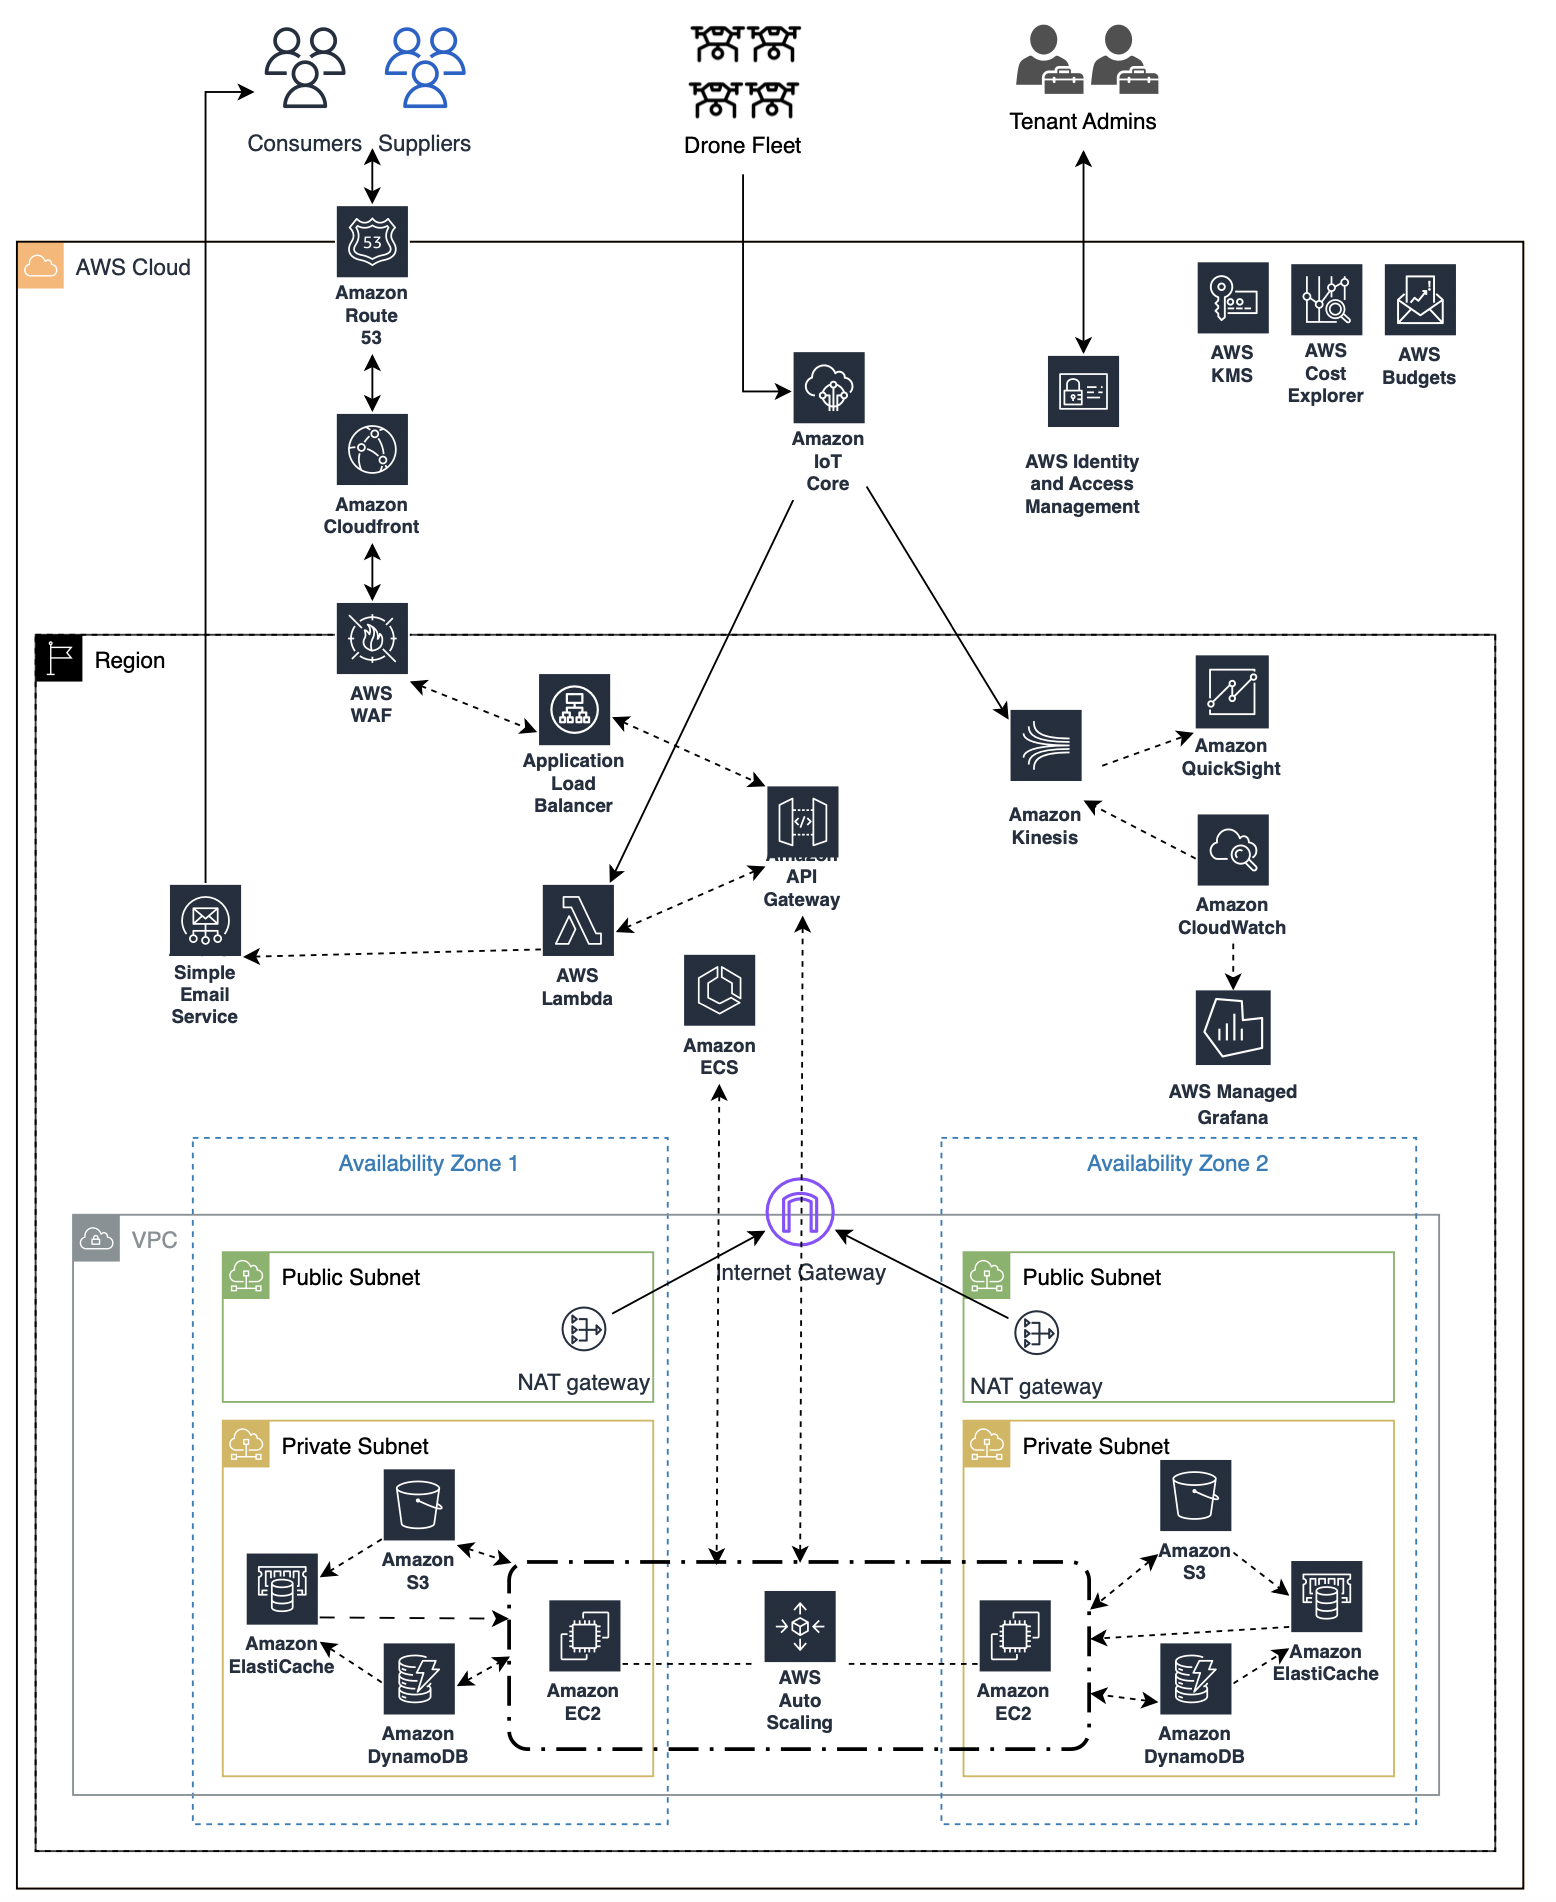
\includegraphics[width=1.1\linewidth]{images/architecture.png}
\end{figure}
In this section, we design the cloud architecture and describe some of the key components of the same. Before we describe the diagram in detail, there are a few points to be noted here:
\begin{enumerate}
    \item It is a multi-region deployment. Only one region is shown here for legibility purposes. But, when actually implemented, the Elastic Disaster Recovery Service would automatically replicate the entire region along with all its components.
    \item The architecture diagram consists of three types of services:
    \begin{itemize}
        \item \textbf{Zonal services:} Zonal services are confined to a specific Availability Zone (AZ) within an AWS Region. They are designed for highly localized applications where low latency and availability are critical. Examples: AWS EC2, AWS ElastiCache, etc.
        \item \textbf{Regional services:} Regional services span an entire AWS Region, providing a broader reach and higher availability compared to zonal services. They are suitable for applications that require consistent performance and fault tolerance across multiple AZs within a Region. Example: AWS Application Load Balancer (ALB), AWS Lambda, etc.
        \item \textbf{Global services:} Global services are available in all AWS Regions, transcending geographical boundaries. They are ideal for applications that require seamless access from anywhere in the world. Examples of global services include: AWS IAM, AWS KMS, etc.
    \end{itemize}
\end{enumerate}
\subsubsection{Users}
We can see from the diagram above that 3 different types of users that interact with our system:
\begin{enumerate}
    \item \textbf{Suppliers and Consumers}: Suppliers are the ones who initiate the package delivery. Consumers are the ones who get the packages through drones. Both of them are crucial stakeholders in our system. 
    \item \textbf{Drone Fleet}: They interact with the system using IoT core service. They receive important insights from the service and publish their status to the service. 
    \item \textbf{Tenant Admins}: They are the ones who would create, manage and maintain the cloud infrastructure, assign roles, allocate quotas, monitor alerts, etc.
\end{enumerate}

\subsubsection{Flows}
\begin{enumerate}
    \item \textbf{Web Application Flow}:
    This flow is mainly meant for suppliers and consumers. They interact with the system using the DNS provided by Route 53 service and reach the fast and scalable CDN provided by CloudFront. This forwards the request to WAF, which sits at the edge of a region. WAF filters out the malicious requests and forwards legitimate requests to Application load balancer, which in-turn passes on the request to the API gateway. The request is then handled by Lambda or EC2 auto scaling group depending on the request. The EC2 instance communicates with S3 and DynamoDB or cache and responds to the requests. If required, the SES service notifies users about the real time updates of the drone fleet. 

    We can see that each of the Availability Zone is divided into a public and a private subnet. The public subnet hosts a NAT Gateway that interacts with the Internet Gateway to communicate with the internet. Notice that this is a unidirectional data flow and external requests are not handled in this flow. The private subnet hosts all the critical compute and storage components.  
    
    \item \textbf{Logging and Monitoring Flow}:
    AWS CloudWatch monitors logs across all the services in a region. These logs are utilized by the Grafana service to create visualizations. They are also passed to Kineses as log streams which then sends them to QuickSight to generate analytics and further visualizations. 
    \item \textbf{IoT service Flow}: \label{iot_flow}
    The drone fleet communicates with the cloud using MQTT by leveraging the IoT core service. These data is passed on as streams to Kineses for generating analytics and visualizations using QuickSight. This event driven flow triggers the lambda functions that enables us to not only monitor the data published by the drones, but also notify users about the latest updates. 
    We can also see a connection between the lambda function that receives data from IoT core service and API Gateway. This facilitates our delayed data collection. If the drones publish the data in a delayed fashion, our APIs can get the same stored into our database. 
\end{enumerate}


\subsection{Validation of the design}
 Now that we have designed the architecture, in this section, we revisit the TRs and validate each TR against our design. We mention the services satisfying the TR and justify the same. \\
 \textit{Note: You might not see all the (repetitive) TRs as although each TR deserved a justification as to why it satisfies the BR, we thought it was redundant to list and justify the services for the same TR twice if it appears. }
\begin{table}[H]
    \centering
    \def\arraystretch{1.75}
    \begin{tabular}{|p{0.2\linewidth}| p{0.3\linewidth} | p{0.5\linewidth} |} \hline 
         \textbf{Business Requirements} &  \textbf{Technical Requirements} & \textbf{Associated Service(s) and Justification}\\ \hline 
         \textbf{[BR1]} Optimize cost &  \textbf{[TR1.1]} 
         
         Implement Auto-Scaling &  We have used the AWS Auto Scaling service along with AWS Application Load balancer to implement Auto-Scaling. Some of the logic is handled by AWS Lambda which is inherently scalable on-demand.  \\ \hline 
         &  \textbf{[TR1.2]} Setup workload monitoring and  
         prediction &  As we can see from the diagram, we have setup AWS CloudWatch along with Grafana, Kineses and  QuickSight to generate, monitor and visualize logs. QuickSight also generate other important business analytics helpful for the stakeholders to make informed decisions. \\ \hline 
         &  \textbf{[TR1.3]} Health Checks & AWS CloudWatch implements health checks using a combination of monitoring agents, data collection. \\ \hline 
         &  \textbf{[TR1.4]} Budgeting alerts & We can see in the global services that AWS Cost Explorer and AWS Budgets have been setup to effectively monitor costs and send out budgeting alerts. \\ \hline 
         \textbf{[BR2]} Tenant Identification &  \textbf{[TR2.1]} Multi-Tenancy Architecture &  We have used services like AWS EC2, DynamoDB and Lambda that facilitates us in creating multi-tenant isolated architectures. EC2 instances and/or Lambda functions can be isolated among tenanats using IAM roles and policies to control access to resources.\\ \hline 
         &  \textbf{[TR2.2]} Identity and Access Management (IAM) &  As seen in the diagram, we use AWS IAM to manage roles and fine grained access to various cloud infrastructure.  \\  \hline 
         &  \textbf{[TR2.3]} Authentication and Authorization Services &  So far as the atchitecture itself is concerned, IAM does the authorization. For the web application, our APIs will handle the same at code level. We may rely on open sources authentication providers like Keycloak for the same. \\ \hline 
         \textbf{[BR3]} Real time Monitoring and Control &   \textbf{[TR3.1]} Establish MQTT communication channel(s) & We leverage AWS IoT Core and AWS Kineses service to establish a publish-subscribe based communication mechanism with the drone fleet. This enables us to send, receive and efficiently process virtually billions of messages.  \\ \hline 
         &  \textbf{[TR3.2]} Implement logging &  Logging plays a crucial part in monitoring. AWS CloudWatch logs all the critical and non-critical events happening across the entire cloud infrastructure. Combining the same with Grafana gives us the ability to monitor logs and visualize the same in real time. \\ \hline 
    \end{tabular}
\end{table}

\begin{table}[H]
    \centering
    \def\arraystretch{1.75}
    \begin{tabular}{|p{0.2\linewidth}| p{0.3\linewidth} | p{0.5\linewidth} |} \hline 
         \textbf{Business Requirements} &  \textbf{Technical Requirements} & \textbf{Associated Service(s) and Justification}\\ \hline 
         \textbf{[BR4]} Customer Engagement&  \textbf{[TR4.1]} Update status of deliveries in real time on customer dashboard. & We use highly efficient Content Delivery Networks like AWS CloudFront to build and deliver the contents on a dashboard for customers. This way, both the suppliers and consumers can get updates in (near) real-time about the drone deliveries.   
         \\ \hline
          &  \textbf{[TR4.2]} Implement email / notification delivery service &  As we can see, some of the events generated by the lambda service trigger email notifications to the customers using the AWS SES service. \\ \hline 
          
            \textbf{[BR5]} Performance Measurement&  \textbf{[TR5.1]} Enable monitoring and generate analytics & We generate analytics and monitor the results and insights using services like AWS QuickSight and AWS Managed Grafana.\\ \hline
         % &  \textbf{[TR5.2]} Implement logging &  \\ \hline
         \textbf{[BR6]} Data Security&  \textbf{[TR6.1]} Keep data encrypted & We use AWS EKS service combined with AWS DynamoDB and AWS S3 to keep the data encrypted. \\ \hline
         &  \textbf{[TR6.2]} Implement rate limiting (1000 requests/second)& AWS Web Application Firewall helps us with rate limiting. We can define custom policies to allow/deny requests.\\ \hline
         % &  \textbf{[TR6.3]} Health Checks &  \\ \hline
         % &  \textbf{[TR6.4]} Implement logging & \\ \hline
         &  \textbf{[TR6.5]} Setup distributed architecture &  We can see in the diagram that we have setup a distributed architecture by deploying services in multiple availability zones and regions.\\ \hline
         \textbf{[BR7]} Continuous Service Improvement&  \textbf{[TR7.1]} Enable monitoring and generate analytics & The analytics generated by AWS QuickSight will be analyzed by the admins that can help in continuous service improvement.   \\ \hline
         % &  \textbf{[TR7.2]} Health Checks & \\ \hline

         % &  \textbf{[TR7.3]} Implement logging & \\ \hline
         % &  & \\ \hline
%     \end{tabular}
% \end{table}

% \begin{table}[H]
%     \centering
%     \def\arraystretch{1.75}
%     \begin{tabular}{|p{0.2\linewidth}| p{0.3\linewidth} | p{0.5\linewidth} |} \hline 
         % \textbf{Business Requirements} &  \textbf{Technical Requirements} & \textbf{Associated Service(s) and Justification}\\ \hline 
         % \textbf{[BR8]} High Availability&  \textbf{[TR8.1] } Implement Auto-Scaling& \\ \hline
         % &  \textbf{[TR8.2]} Setup workload monitoring and prediction& \\ \hline
         % &  \textbf{[TR8.3]} Implement rate limiting & \\ \hline
         \textbf{[BR8]} High Availability &  \textbf{[TR8.4]} Implement version control & We have used AWS ECS service to manage containers for the images. We can version images by release tags. This can help us roll-back to previous stable releases in case of failures in newer ones. \\ \hline
         &  \textbf{[TR8.5]} Enable disaster management and recovery & We store backups in S3 Buckets. We deploy the infrastructure in multiple availability zones, thereby ensuring disaster management and recovery\\ \hline
         % &  \textbf{[TR8.6]} Health checks& \\  \hline
         % &  \textbf{[TR8.7]} Implement logging& \\ \hline
         % &  \textbf{[TR8.8]} Setup distributed architecture& \\ \hline
         \textbf{[BR9]} Delayed Data Collection&  \textbf{[TR9.1]} Automated data synchronization& We use services like AWS IoT core that leverages Publish Subscribe mechanism. As mentioned in the IoT Service flow [\ref{iot_flow}], we leverage this to ensure automated data synchronization and hence enable delayed data collection. \\ \hline
    \end{tabular}
\end{table}

\newpage
\subsection{Design principles and best practices used}
\subsubsection{Design Principles}
\begin{enumerate}
    \item \textbf{Perform operations as code \cite{Opex}:} We use AWS Lambda alongside Amazon API Gateway to automate our operations, which aligns with our goal for real-time monitoring \textbf{(TR3.2)}. This ensures that our responses to events are consistent and error-free, leveraging the power of code to define and update our workload.
    \item \textbf{Make frequent, small, reversible changes \cite{Opex}:} We have  used AWS Auto Scaling and Amazon EC2 which allows us to implement incremental changes, thereby enhancing our system's scalability \textbf{(TR1.1)}. This approach not only reduces risk but also empowers us to adapt swiftly to evolving requirements.
    \item \textbf{Anticipate failure \cite{Opex}:} We have utilized the combination of Amazon CloudWatch and Amazon S3 to proactively monitor address failures \textbf{(TR7.2)}, constantly refining our operational procedures to mitigate risks before they impact our services.
    \item \textbf{Automatically recover from failure \cite{rel}:} We've configured AWS CloudWatch to initiate automatic recovery processes (TR8.6), with Amazon S3 serving as our resilient backup and recovery solution, guaranteeing continuous service availability.
    \item \textbf{Test recovery procedures \cite{rel}:} We regularly test our recovery strategies (TR7.3) using AWS Lambda and Amazon EC2, ensuring our services can quickly rebound from disruptions and maintain reliability.
    \item \textbf{Scale horizontally \cite{rel}:} Our architecture is designed to distribute operations across multiple Amazon EC2 instances (TR8.1), utilizing AWS Auto Scaling to maintain high availability and fault tolerance.
    \item \textbf{Implement cloud financial management \cite{Cost dp}:} We have used tools like AWS Cost Explorer and AWS Budgets which are central to our financial management strategy \textbf{(TR1.4)}, helping us to monitor and optimize our spending effectively.
    \item \textbf{Adopt a consumption model \cite{Cost dp}:} Our use of AWS Lambda and AWS Auto Scaling reflects our commitment to a consumption-based model (TR1.1), where we scale our resources to match demand, ensuring we pay only for the resources we need.
    \item \textbf{Measure overall efficiency \cite{Cost dp}:} We apply Amazon QuickSight and AWS Managed Grafana (TR5.1) to measure our workload's efficiency, ensuring that we deliver value while managing our costs prudently.

\end{enumerate}

\subsubsection{Best Practices}
\begin{enumerate}
    \item \textbf{Prepare, Operate, Evolve}  \cite{prepare}\cite{operate}\cite{evolve}\\\\
    We have employed budgeting alerts to enhance our operational excellence. By doing so, we are not only prepared to manage our financial resources but also have a system that evolves with our spending patterns, ensuring that we stay within budget while maximizing the capabilities of AWS. This approach exemplifies our commitment to maintaining operational discipline and enhancing the predictability of our operational expenses.\\\\
    \textbf{TR Satisfied -} TR1.4 Budgeting alerts.
    \item \textbf{Identity and Access Management} \\\\
    We've implemented a robust multi-tenancy architecture and identity management system, which are foundational to our security posture. Through these implementations, we ensure that each user and service operates with the minimum necessary privileges, enhancing the security of our system and protecting our resources from unauthorized access. This not only strengthens our compliance with the principle of least privilege but also underpins our entire security strategy.\\\\ 
    \textbf{TRs Satisfied -} TR2.1 Multi-Tenancy Architecture, TR2.2 IAM
    \item \textbf{Infrastructure Protection}\cite{Infrastructure protection} \\\\
    We have adopted a distributed architecture to protect our infrastructure, which aligns with the reliability pillar of the framework. This setup enables us to distribute our workload across multiple resources, avoiding single points of failure and significantly reducing the potential impact of outages or attacks, thereby reinforcing our system's resilience and operational stability.\\\\
    \textbf{TR Satisfied -} TR8.8 Setup distributed architecture
    \item \textbf{Data Protection}\cite{Data protection} \\\\
    We have employed AWS Key Management Service (KMS) and advanced data encryption techniques to meticulously classify and encrypt our data, both at rest and in transit. This practice is fundamental in ensuring that sensitive information is rigorously protected, thereby meeting the highest standards of confidentiality and integrity as mandated by the security pillar of the AWS Well-Architected Framework.\\\\
    \textbf{TR Satisfied -} TR6.1 Keep data encrypted
    \item \textbf{Incident Response}\cite{Incident response} \\\\
    We have developed a comprehensive incident response plan, bolstered by extensive logging mechanisms using services like Amazon CloudWatch and QuickSight. These tools enable us to rapidly detect and respond to incidents, ensuring minimal impact on our operations. Our approach to logging goes beyond merely recording events; it is an integral part of our strategy for quickly understanding and addressing potential security issues, leveraging the advanced capabilities of Amazon CloudWatch and QuickSight for real-time analysis and insights.\\\\
    \textbf{TR Satisfied -} TR7.3 Implement logging
     \item \textbf{Failure Management}\cite{Failure management} \\\\
    We've implemented a robust disaster recovery strategy, essential for managing and recovering from system failures. This strategy includes regularly backing up our data to alternate S3 and DynamoDB locations and rigorously testing our recovery procedures. Such practices underscore our dedication to providing a reliable and resilient cloud service.\\\\
    \textbf{TR Satisfied -} TR8.5 Enable disaster management and recovery
    \item \textbf{Foundations}\cite{Foundations} \\\\
    We have laid strong foundations for reliability by implementing sophisticated workload monitoring and predictive scaling. These practices ensure we can dynamically adapt our resources to meet the demands of our workload, preventing over-provisioning and undersupply, thus maintaining our system's reliability even as demand fluctuates.\\\\
    \textbf{TR Satisfied -} TR8.2 Setup workload monitoring and prediction
    \item \textbf{Monitoring}\cite{monitoring} \\\\
    We've strategically utilized AWS QuickSight and Grafana to enhance our monitoring capabilities. QuickSight allows us to create intuitive and interactive data visualizations, crucial for understanding our workload and making informed decisions. Grafana, on the other hand,  complements this by offering in-depth analysis and observability. This combination empowers us to not only monitor our resources efficiently but also to transform vast datasets into actionable insights, ensuring that our resources are optimized for both performance and cost\\\\
    \textbf{TR Satisfied -} TR5.1 Enable monitoring and generate analytics
    \newpage
    \item \textbf{Expenditure Awareness}\cite{Expenditure and usage awareness} \\\\
    We maintain a high level of expenditure awareness by employing AWS budgeting alerts. This vigilant approach to cost management ensures that we are always informed about our spending and can make timely adjustments to stay aligned with our financial objectives.\\\\
    \textbf{TR Satisfied -} TR1.4 Budgeting alerts

    \item \textbf{Matching Supply \& Demand}\cite{Manage demand and supply resources} \\\\
   We have expertly matched the supply of resources with demand by leveraging AWS Auto-Scaling. This ensures that we can seamlessly handle traffic spikes and lulls, maintaining optimal performance and cost-effectiveness.\\\\
    \textbf{TR Satisfied -} TR1.1 Implement Auto-Scaling

    
    
\end{enumerate}


\subsection{Trade offs revisited}
\begin{enumerate}
    \item \textbf{\ref{BR1 - Optimize costs} Optimize costs vs. \ref{BR8 - High Availability} High availability}: \textbf{[SELECTED: HIGH AVAILABILITY]}\\\\
    Cost optimization (BR1) is fundamental to operating sustainably, especially in a competitive market. It involves careful resource allocation and scaling to avoid unnecessary expenditure. However, the importance of high availability (BR8) cannot be understated, as it ensures service reliability and customer satisfaction. \\\\
    We have used AWS services such as AWS Auto Scaling, Amazon EC2, and Amazon Route 53 to strike a balance between cost optimization (BR1) and high availability (BR8). While AWS Auto Scaling dynamically adjusts resources to maintain optimal cost efficiency, strategies like deploying across multiple Availability Zones with Amazon EC2 and using Route 53 for DNS failover mechanisms increase availability. The trade-off generally favors high availability, as the drone delivery service is highly dependent on constant uptime to maintain service levels and customer trust. Costs are managed by scaling down resources during low demand and employing cost-effective services like Amazon S3 for storage, but the architecture is designed to prioritize availability even if it incurs additional costs. The rationale is that the cost of downtime, both in terms of direct revenue loss and reputational damage, can far outweigh the expenses incurred in maintaining redundant systems and resources.

    \item \textbf{\ref{BR6 - Data Security} Data security vs. \ref{BR9 - Delayed Data Collection} Delayed Data Collection}: \textbf{[SELECTED: DATA SECURITY]}\\\\
    Data security (BR6) is paramount, as it protects sensitive customer information and maintains trust. AWS KMS is used to ensure data encryption, while AWS IoT Core manages secure data transfer. On the other hand, timely data collection (BR9) is essential for operational efficiency and service responsiveness. AWS Lambda can process and synchronize data efficiently when connectivity is established.\\\\
    Data security is non-negotiable, particularly when handling sensitive customer information. Thus, even though drones may experience intermittent connectivity, the architecture ensures that any data collected is encrypted at rest using AWS KMS, and transferred securely using protocols supported by AWS IoT Core. Delayed data collection is managed by storing data locally on drones in a secure manner and synchronizing it with the cloud as soon as connectivity is restored. Security measures are meticulously implemented and monitored, emphasizing their supremacy in the trade-off. The justification is that any compromise on security could lead to legal and reputational repercussions that could jeopardize the entire service, whereas delays in data collection are often a tolerable inconvenience by comparison.


\end{enumerate}

\subsection{Discussion of an alternate design \color{red}[Skipped]}

\newpage
\section{Kubernetes experimentation}
\subsection{Experiment Design}
In this experiment, we choose a different application for the demonstration used in this section. Before describing the experiment design for kubernetes, let us briefly describe the application that we are going to deploy and come up with a few relevant TRs from the same. 
\subsubsection{The Application}
For the sake of simplicity, we deploy an open source application called NextCloud on AWS EKS cluster.
Below are the technical requirements we will be working with during this experiment.
\subsubsection{Technical Requirements}
\begin{enumerate}[label=\textbf{[TR\arabic*]}, leftmargin=4\parindent]
        \item Use of container orchestration
        \item Implement auto-scaling using kubernetes HPA.
        \item Average CPU Utilization of 50\% should trigger auto-scaling
\end{enumerate}
\subsubsection{Components and Tools}
In this experiment, we will be using the below components and tools:
\begin{itemize}
    \item \textbf{NextCloud App: } Nextcloud is a self-hosted file-sync and cloud storage platform that gives us control over our data. It is a free and open-source alternative to popular cloud storage services like Dropbox and Google Drive. Nextcloud can be used to store and share files, sync files across devices, and collaborate on documents. \cite{nextcloud}
    \item \textbf{Amazon EKS (Elastic Kubernetes Service): } The cloud platform for orchestrating and managing containerized applications.
    \item \textbf{Kubernetes: }Container orchestration tool to manage and deploy application containers.
    \item \textbf{Locust: } Open-source load testing tool to simulate user traffic and generate load.
\end{itemize}
\subsubsection{Description}
This experiment was done by leveraging the above mentioned components and tools. The objective of this experiment is to assess the scalability and performance of an application hosted on Amazon EKS using Kubernetes by simulating varying levels of user load with Locust.
\\\\
In this experiment, the services use a virtual IP address that acts as a single entry point to a group of pods providing the same service. When traffic reaches this service, it is then distributed to individual pods based on the selected load balancing strategy. In our case, we selected an IP-based round robin load balancing technique, where each new connection request is directed to the next available pod IP address in a cyclical manner. Kubernetes utilizes a distributed system approach for load balancing. The control plane components like the node server, scheduler, and controllers are distributed across nodes in the cluster. Additionally, load balancing occurs across multiple pods, which are distributed across different nodes in the cluster, enhancing scalability and fault tolerance.
\\\\
We created a cluster with the default configurations as offered by AWS EKS. Once the cluster was active, we create a managed node group with initial count of 2 nodes, minimum of 2 and a maximum of 5 nodes. The instance types we chose were $t3.micro$ and $t3.medium$. So far as the pods are concerned, we started with conservative resource requests and limits for our pods, with CPU request as 0.2 and memory limit of 200Mi. We used the public \href{https://hub.docker.com/_/nextcloud}{docker image} available for NextCloud and deployed the same on our cluster. 
\newpage
To conduct this experiment, we consider both the cases while deploying the application: 
\begin{itemize}
    \item Without HPA (Horizontal Pod Autoscaler) enabled.
    \item With HPA enabled.
\end{itemize}
For the second part of the experiment, we've set up both Cluster Autoscaling with managed NodeGroups and Horizontal Pod Autoscaling (HPA).
Below is a glimpse of the node autoscaling policy:
\begin{figure}[H]
    \centering
    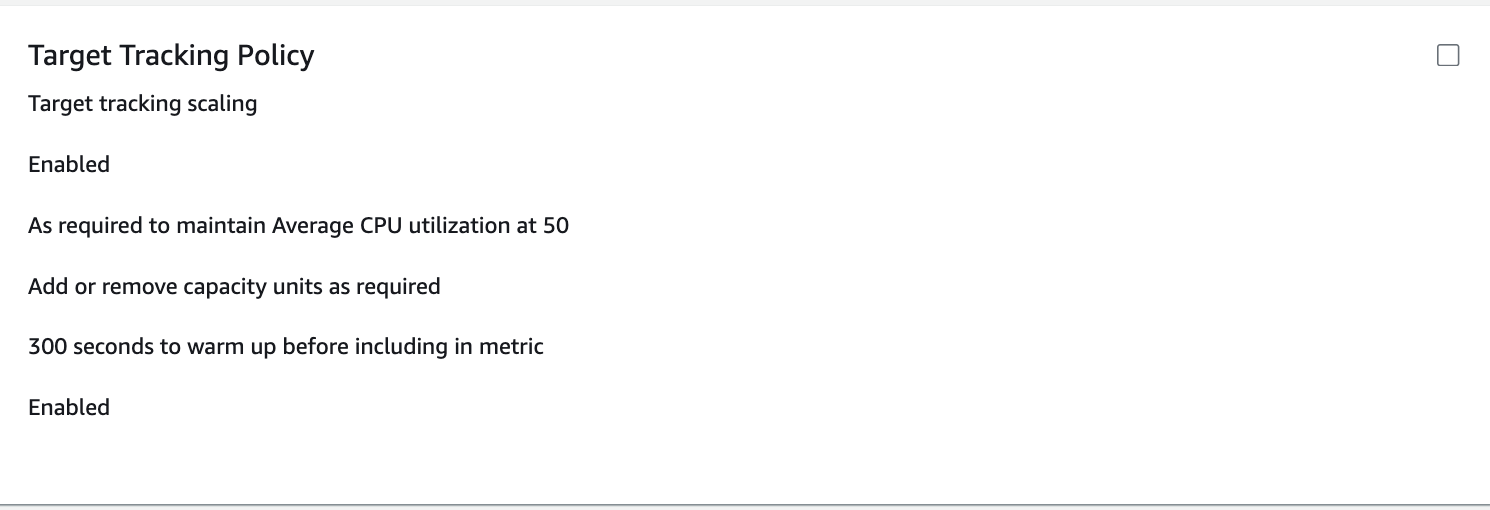
\includegraphics[width=0.75\linewidth]{images/autoscale_nodes.png}
\end{figure}
Cluster Autoscaling dynamically manages the cluster's node count, responding to pod failures or rescheduling onto other nodes [Cluster Autoscaling]. For HPA, we've configured the CPU usage threshold at 50\%. Additionally, we've specified a minimum of 1 pod and a maximum of 5 pods. To provision these resources, we utilized kubectl, Docker, and the AWS Console. So far as the load is concerned, we experiment with 2 different load generation strategies. Initially, we experiment by increasing the load linearly. Upon observing results for a couple of different rates, we experiment with an exponential increase in load. 
Some of the commmands used were as below:
\begin{itemize}
    \item Update $kubectl$ config to point to our cluster:
    \inputminted{sh}{scripts/kubectl_config.sh}
    \item Setup deployment, service, metrics service and autoscaler:
    \inputminted{sh}{scripts/setup.sh}
\end{itemize}
\newpage
We used the below deloyment and service yaml files to setup the cluster:
\begin{figure}[H]
\centering
    \begin{minipage}{0.45\textwidth}
        \inputminted{yaml}{scripts/deployment.yaml}
    \end{minipage}
    \begin{minipage}{0.45\textwidth}
        \inputminted{yaml}{scripts/service.yaml}
    \end{minipage}
\end{figure}

\subsection{Workload generation with Locust}
Locust is an open source load testing framework \cite{locust}, that allows users to define user behaviour with Python code, and swarm our systems with millions of simultaneous users. They offer rich and informative documentation \cite{locust_docs} and is minimalistic, so its really straightforward to work with. \\\\
The fake load was generated using locust. Below is a python code snippet for the same. We can see that we only try to hit the root endpoint '$/$' in the script for the sake of simplicity. The host name was provided in the command to run the locust, or there is an option to update the same in the locust UI as well. 
\inputminted{py}{scripts/locustfile.py}
\subsubsection{Linear}
Locust provides linear increase in load by default. The experiment was performed with the following configurations. 
\begin{figure}[H]
    \centering
    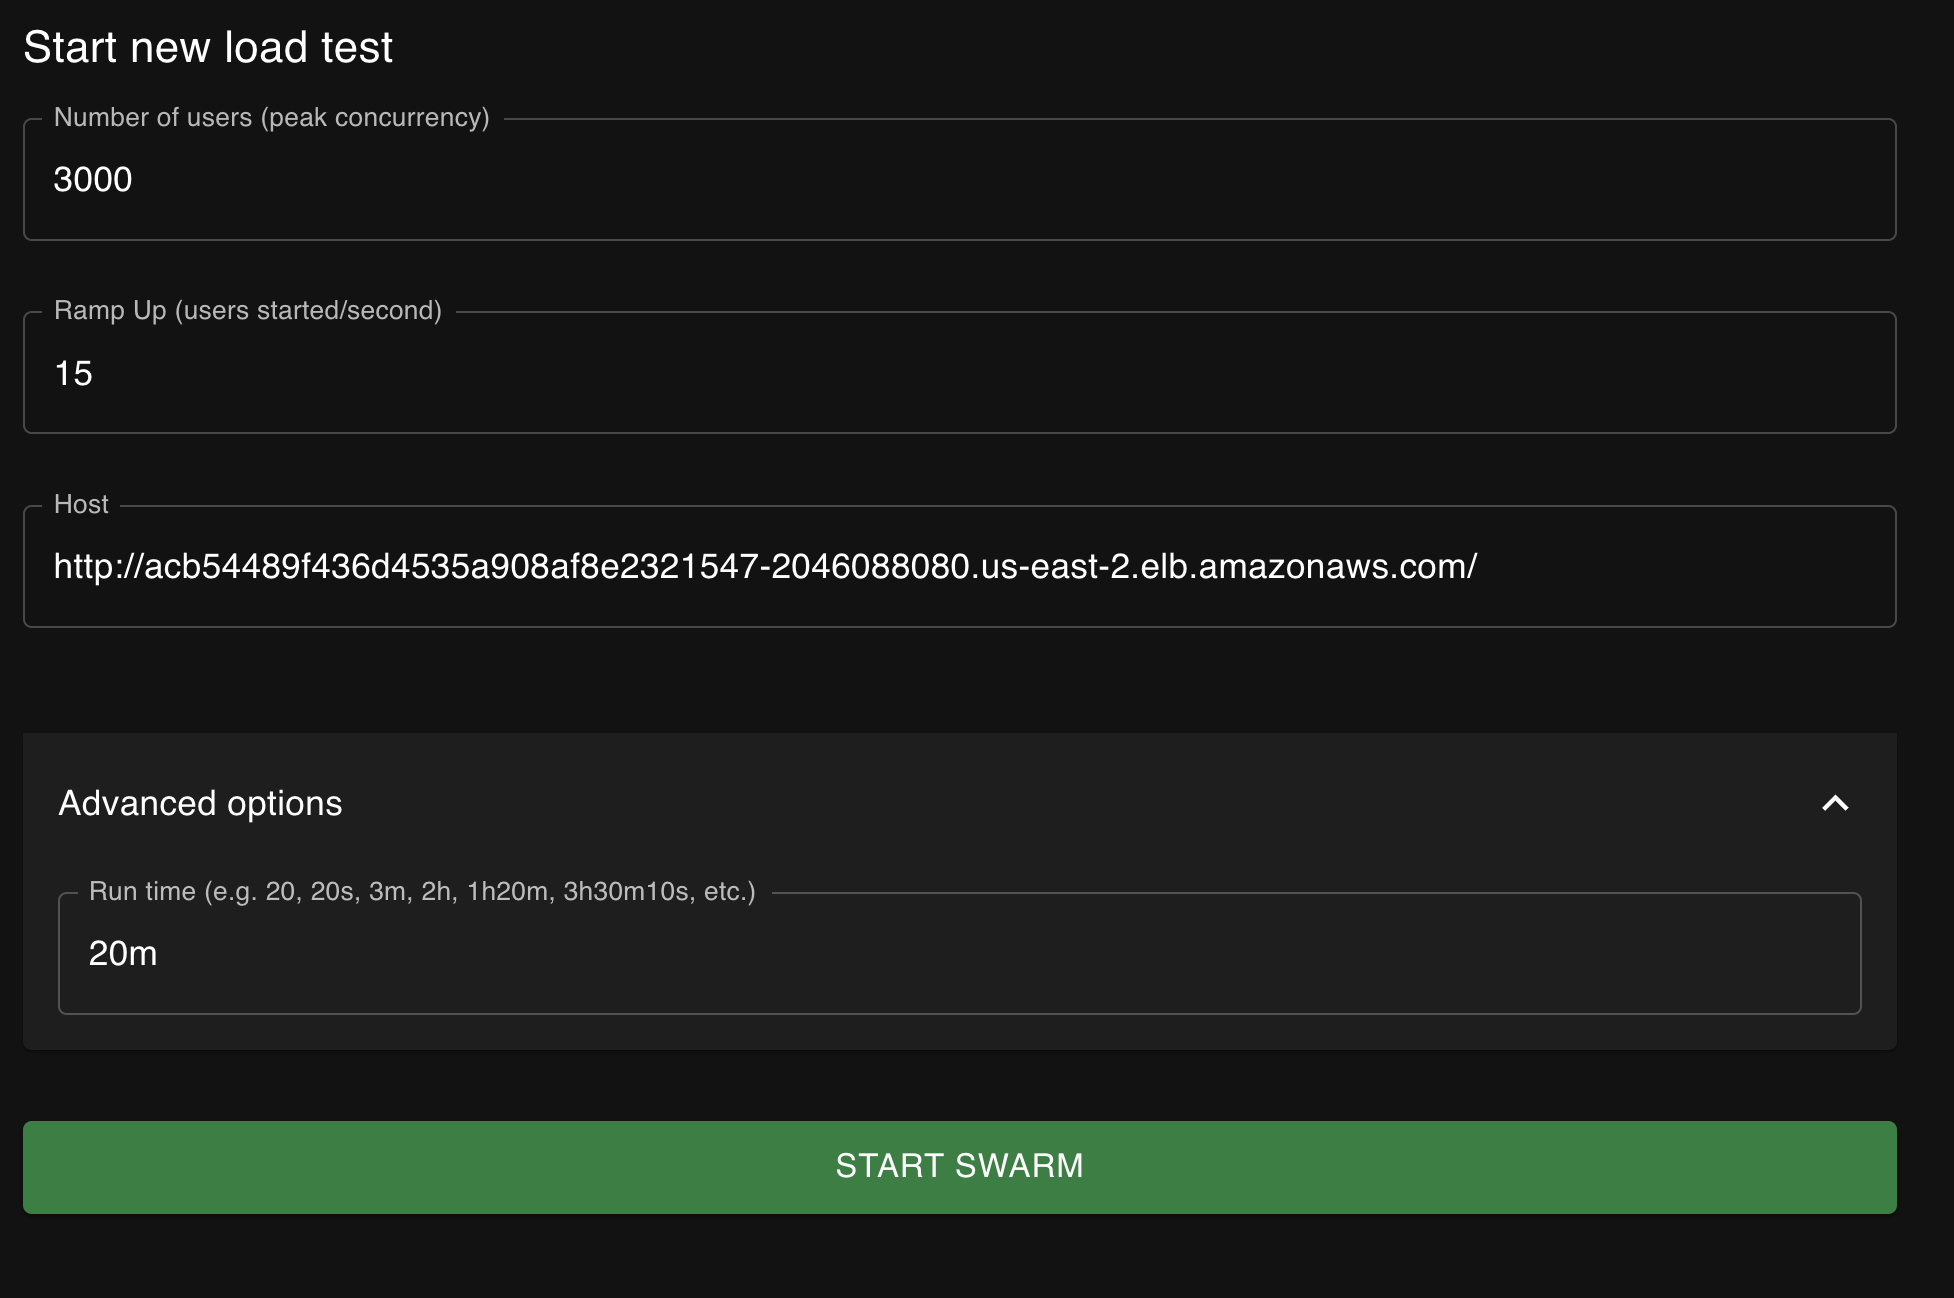
\includegraphics[width=0.75\linewidth]{images/locust_linear.png}
\end{figure}
We can see in the test a linear increase/decrease in the behaviour as below:
\begin{figure}[H]
    \centering
    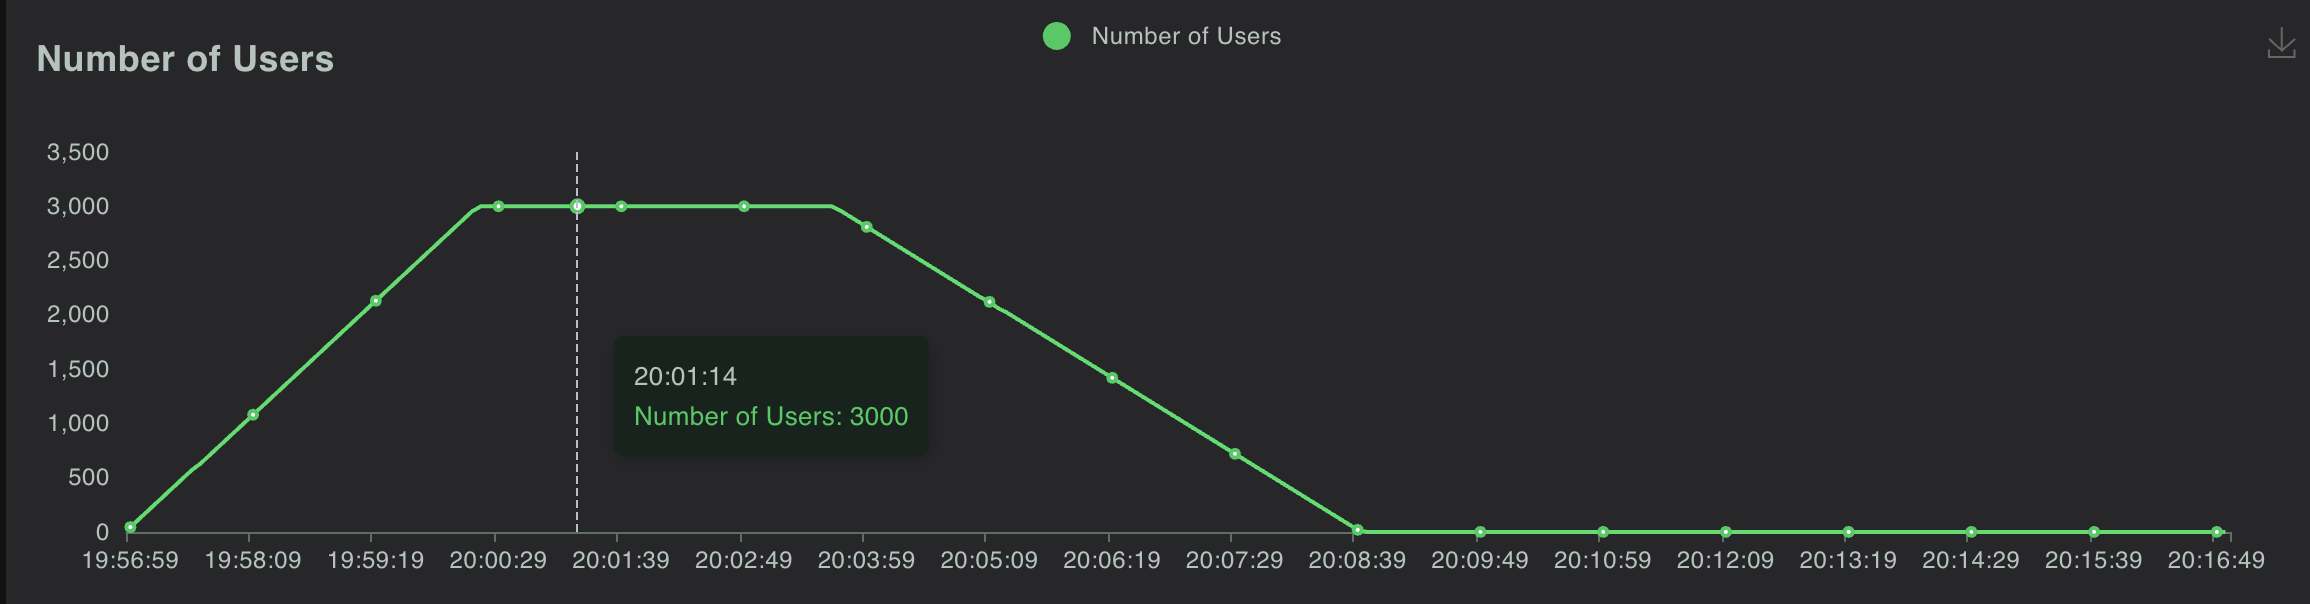
\includegraphics[width=0.9\linewidth]{images/users_linear.png}
\end{figure}
We can also see a linear decrease. That is because we edited the configurations midway to be able to test the scaling down of the autoscaler. We can see that the peak users is 3000.
\subsubsection{Exponential}
Upon looking for a couple of options to vary the load exponentially, we couldn't find much about the same. So, we decided to do an exponential change to the number of users manually. In the locust UI, we get an option to update the configuration in real time. We leveraed the same and varied the users by a factor of 2. We started out by 1 user, and kept increasing by a factor of 2 until a peak of 10000 concurrent users.
\begin{figure}[H]
    \centering
    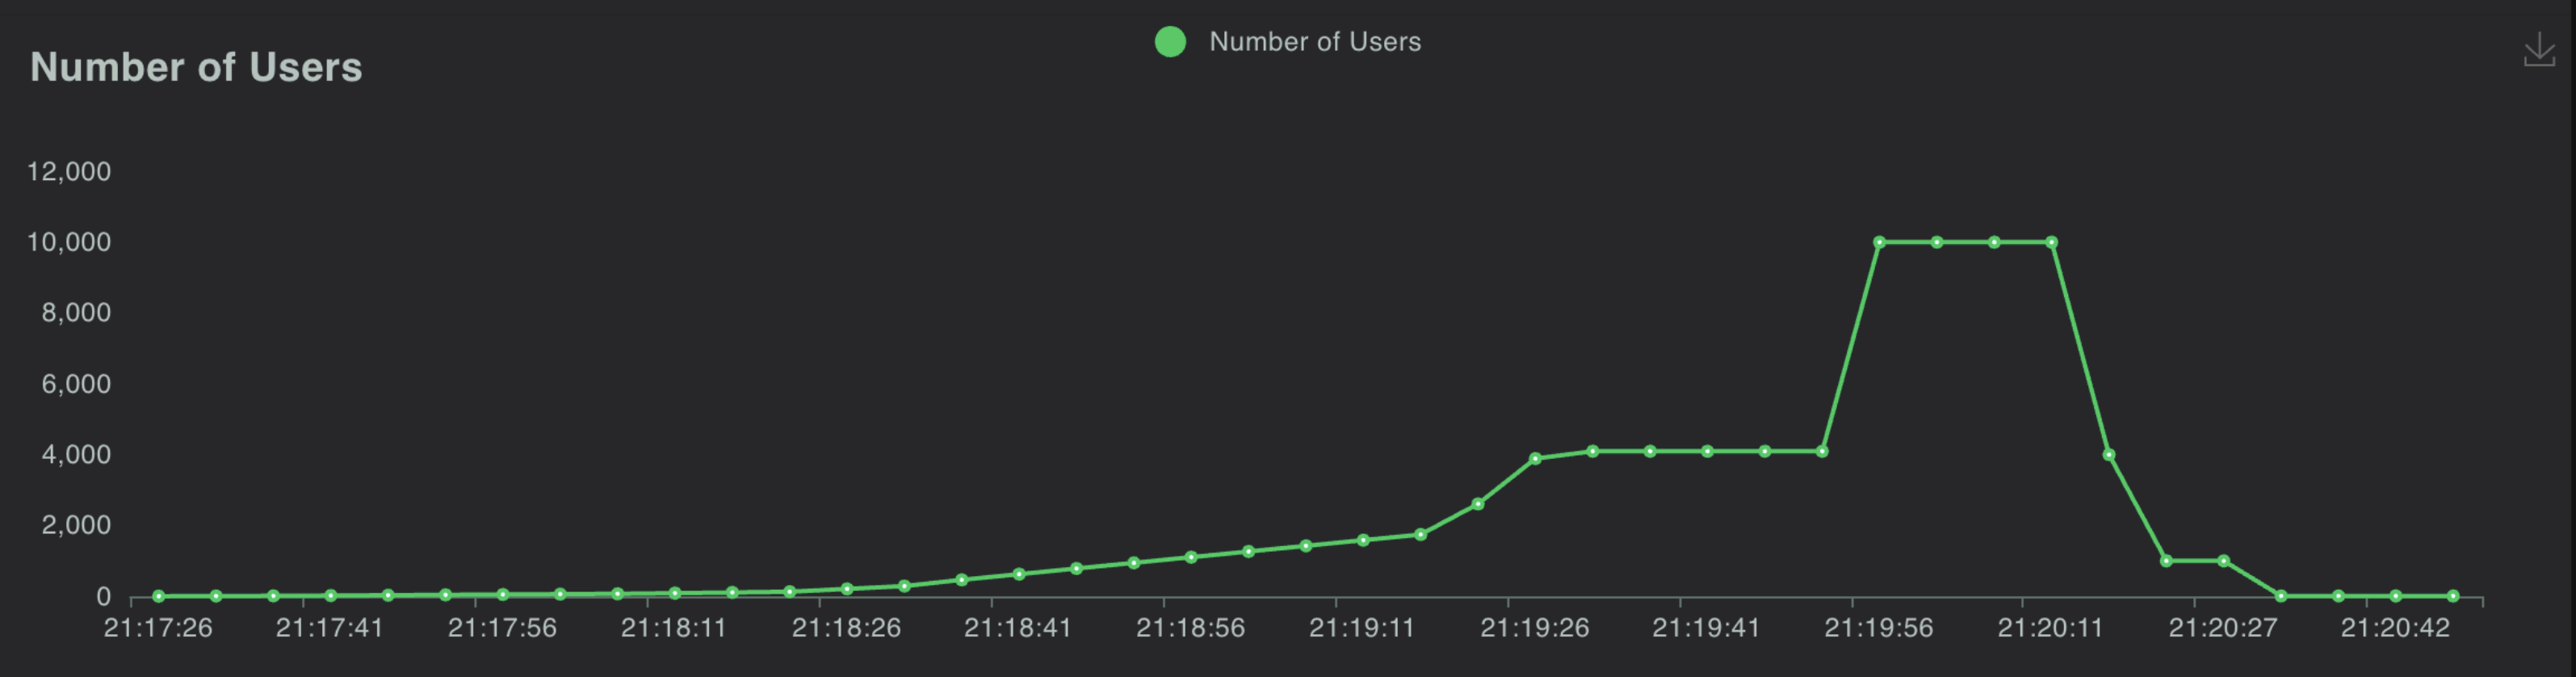
\includegraphics[width=0.9\linewidth]{images/users_exponential.png}
\end{figure}
\subsection{Analysis of the results}
\subsubsection{Experiment 1: Without Auto-Scaling}
In this experiment, we tried to increase the load linearly using locust. Just to get an idea on how does our pods behave when they are not autoscaled, we did not configure the HPA. Below are the results. 
\begin{figure}[H]
    \centering
    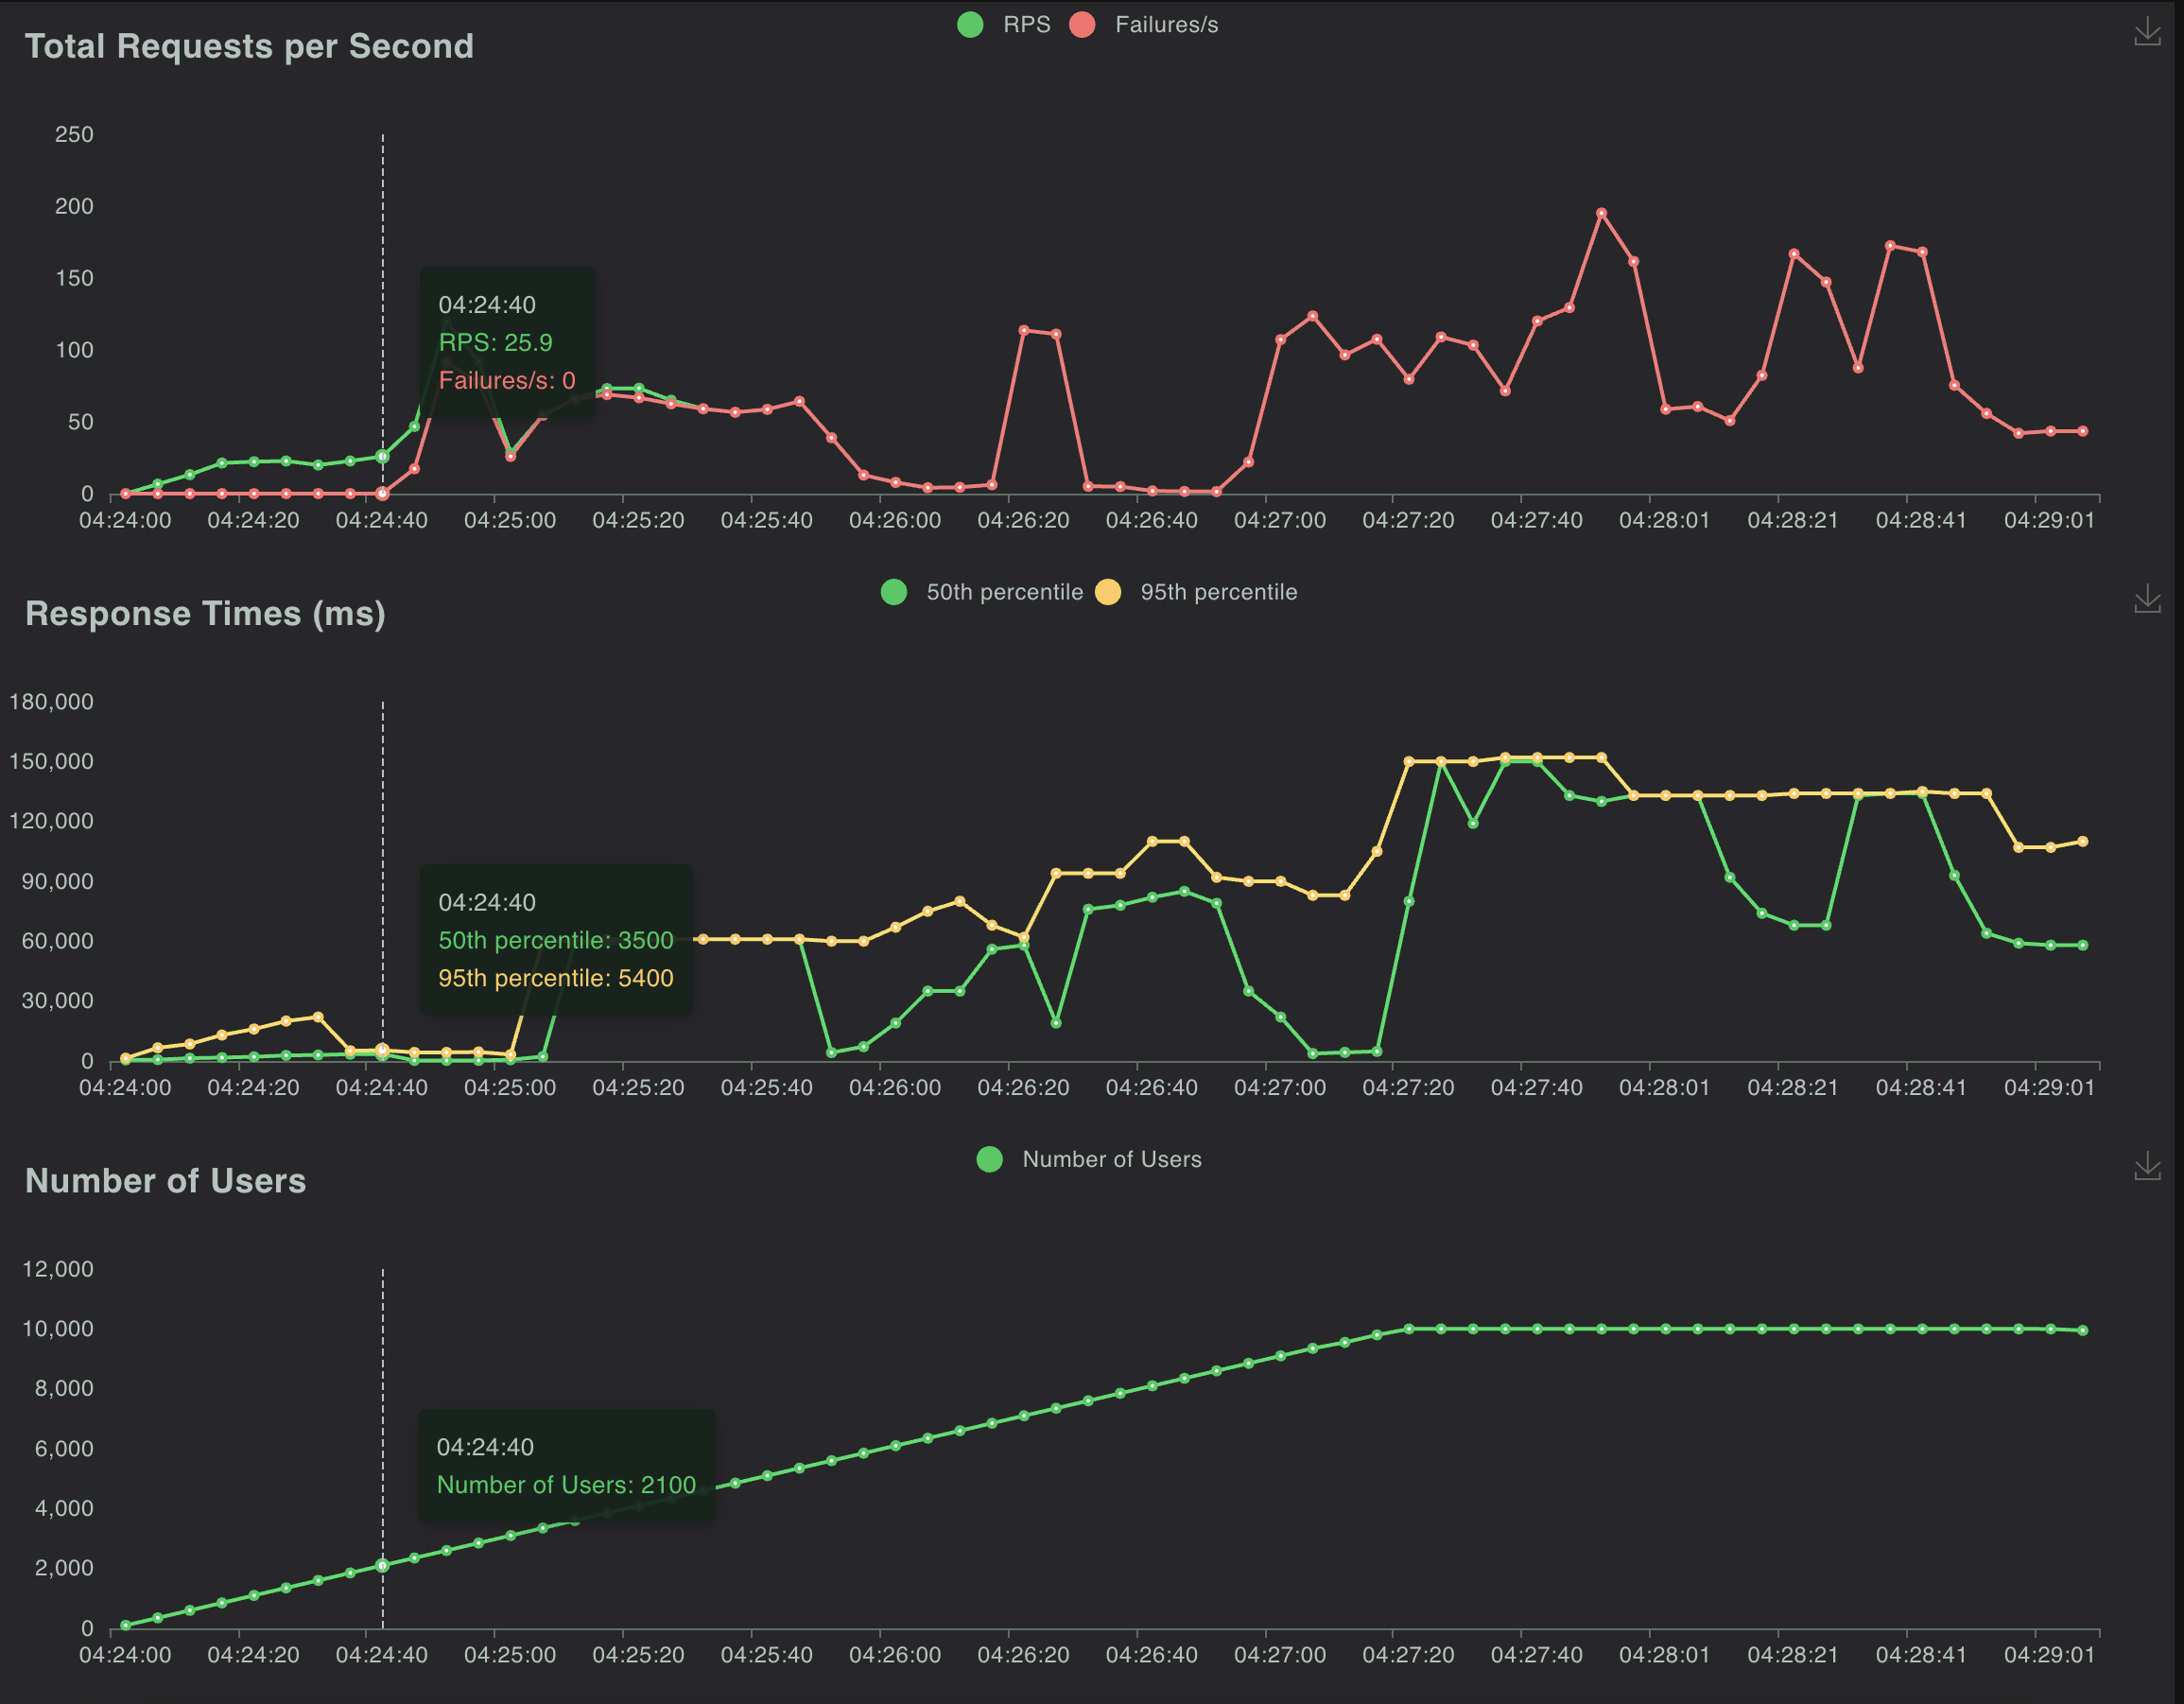
\includegraphics[width=0.9\linewidth]{images/exp1_results.png}
\end{figure}
\begin{figure}[H]
    \centering
    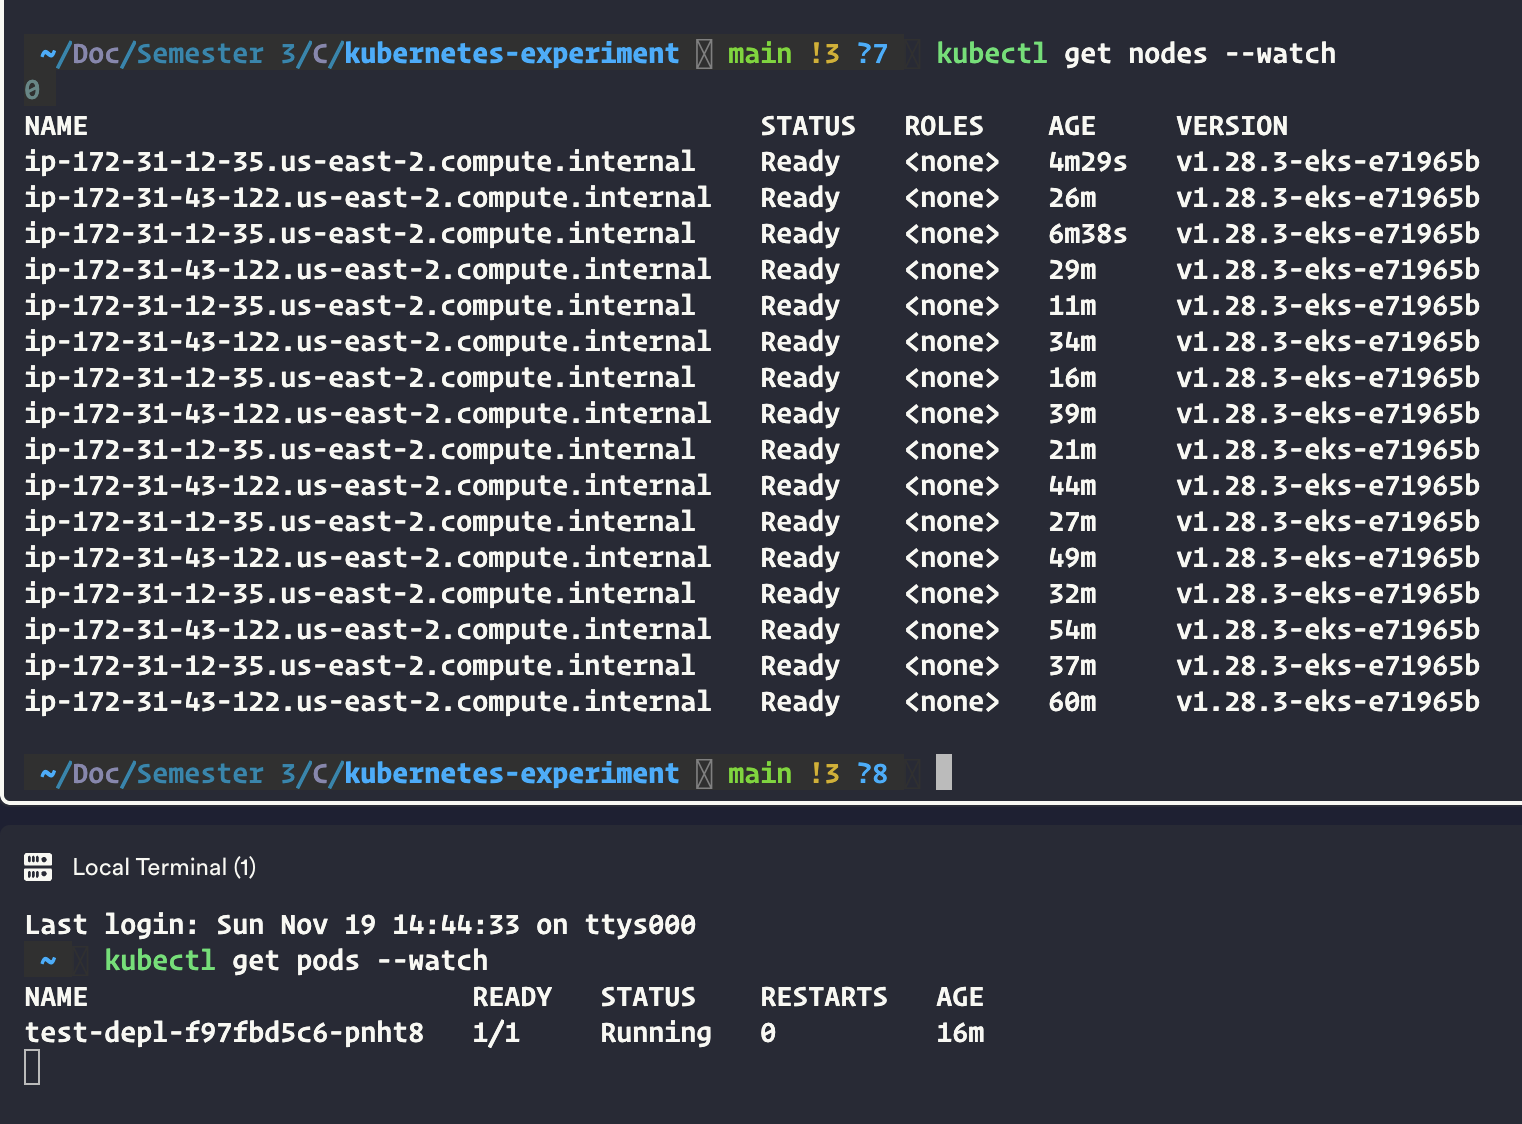
\includegraphics[width=0.7\linewidth]{images/exp1_watch.png}
\end{figure}
As we can see in the above results, the app started giving a bunch of failures when the number of concurrent users reached 2100. Since there was no autoscaling enabled, the pod count remains just 1.  We can also see that there are only 2 instances in the nodes list on top. 

To try out a bit more with better instance, we gave a similar experiment a try with $t3.medium$ instances in the node group. Below are the results for the same. We can now see that the number of concurrent users where failures start kicking in increased from 2100 earlier to almost 6000 in this case. 

This experiment satisfies the TR1 (mentioned above). Even though auto-scaling is not implemented, we have used kubernetes to deploy the app in this experiment. 
\begin{figure}[H]
    \centering
    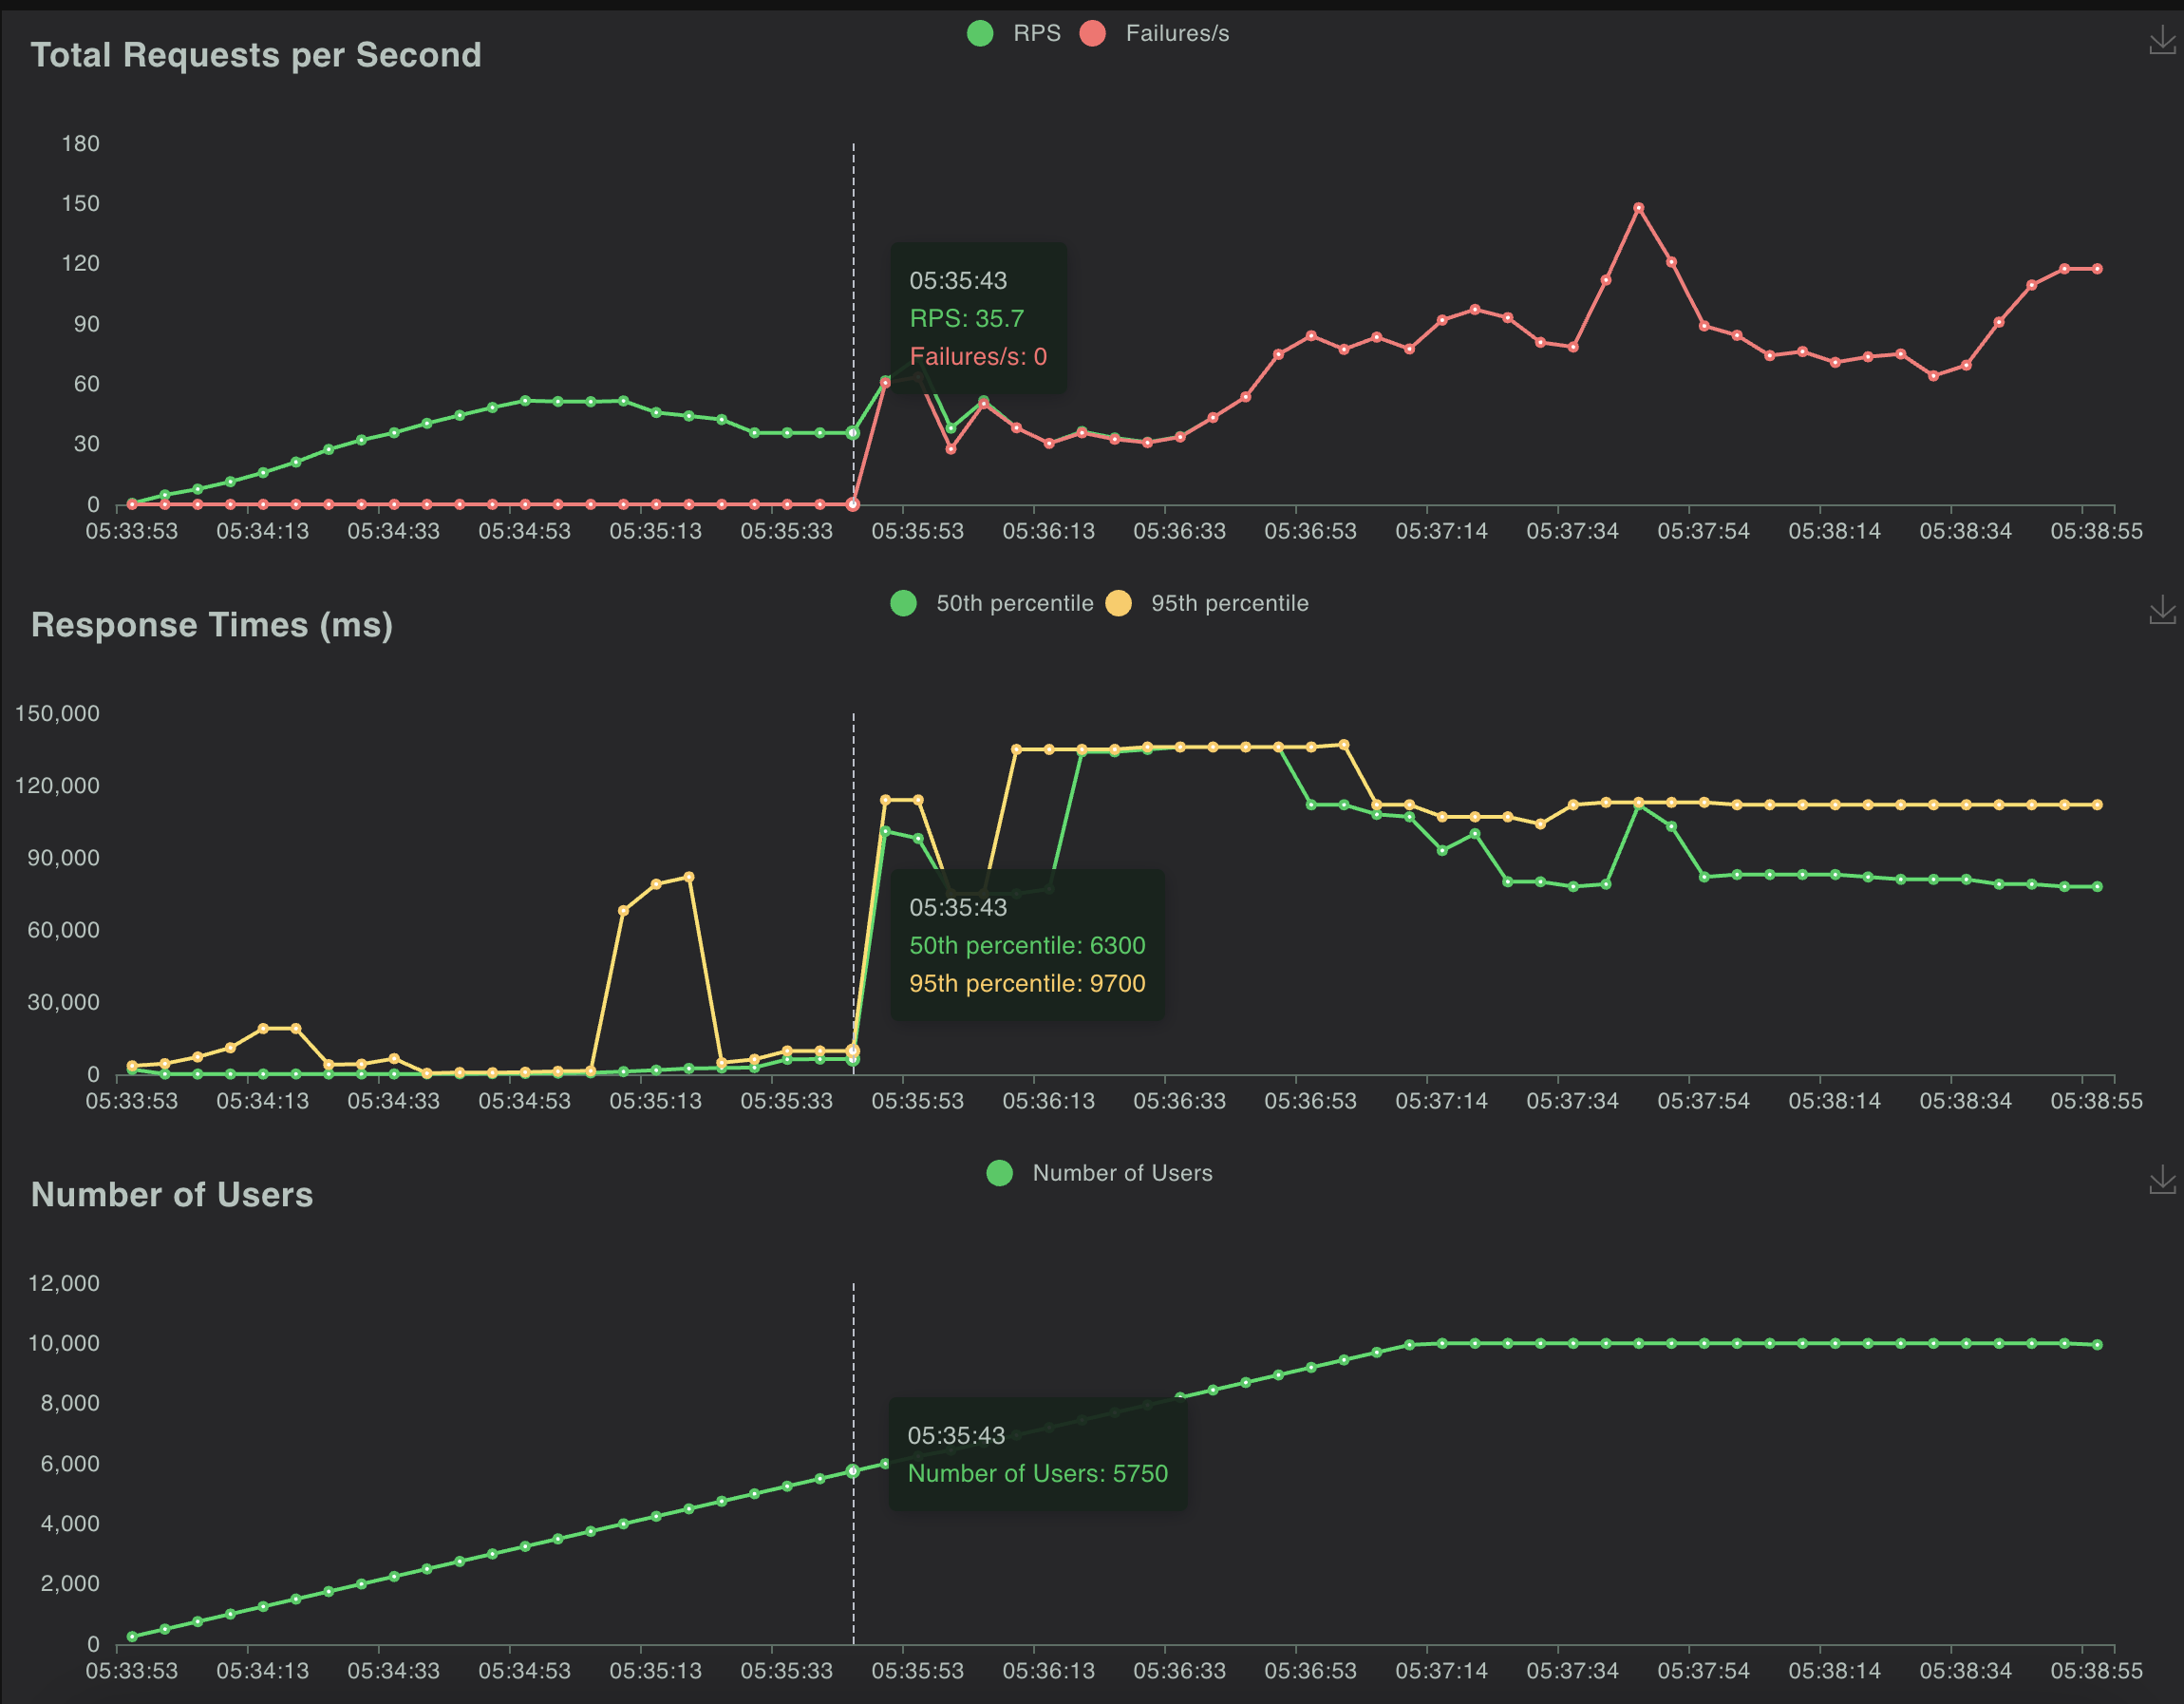
\includegraphics[width=0.9\linewidth]{images/exp_1_2_results.png}
\end{figure}
\newpage
\subsubsection{Experiment 2: With Auto-Scaling (Linear Load)}
In this experiment, we setup the Node Autoscaling along with a Horizontal Pod Autoscaler. We used a linear increase and decrease in the load using locust for the same. Below are the results for the same. Because there was autoscaling enabled, we experimented with $t3.micro$ instace to avoid costs. In this case, we could see the number of pods increasing and decreasing linearly. 
\begin{figure}[H]
    \centering
    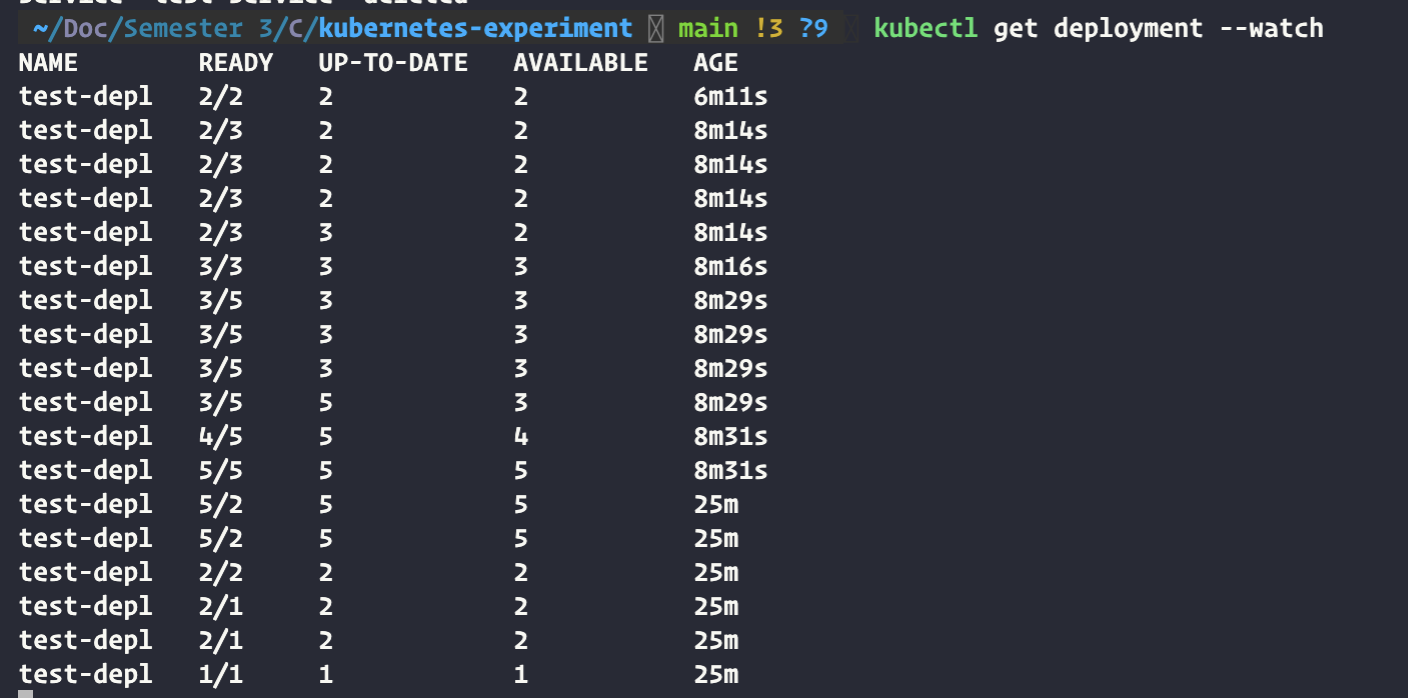
\includegraphics[width=0.7\linewidth]{images/exp2_watch.png}
\end{figure}
\begin{figure}[H]
    \centering
    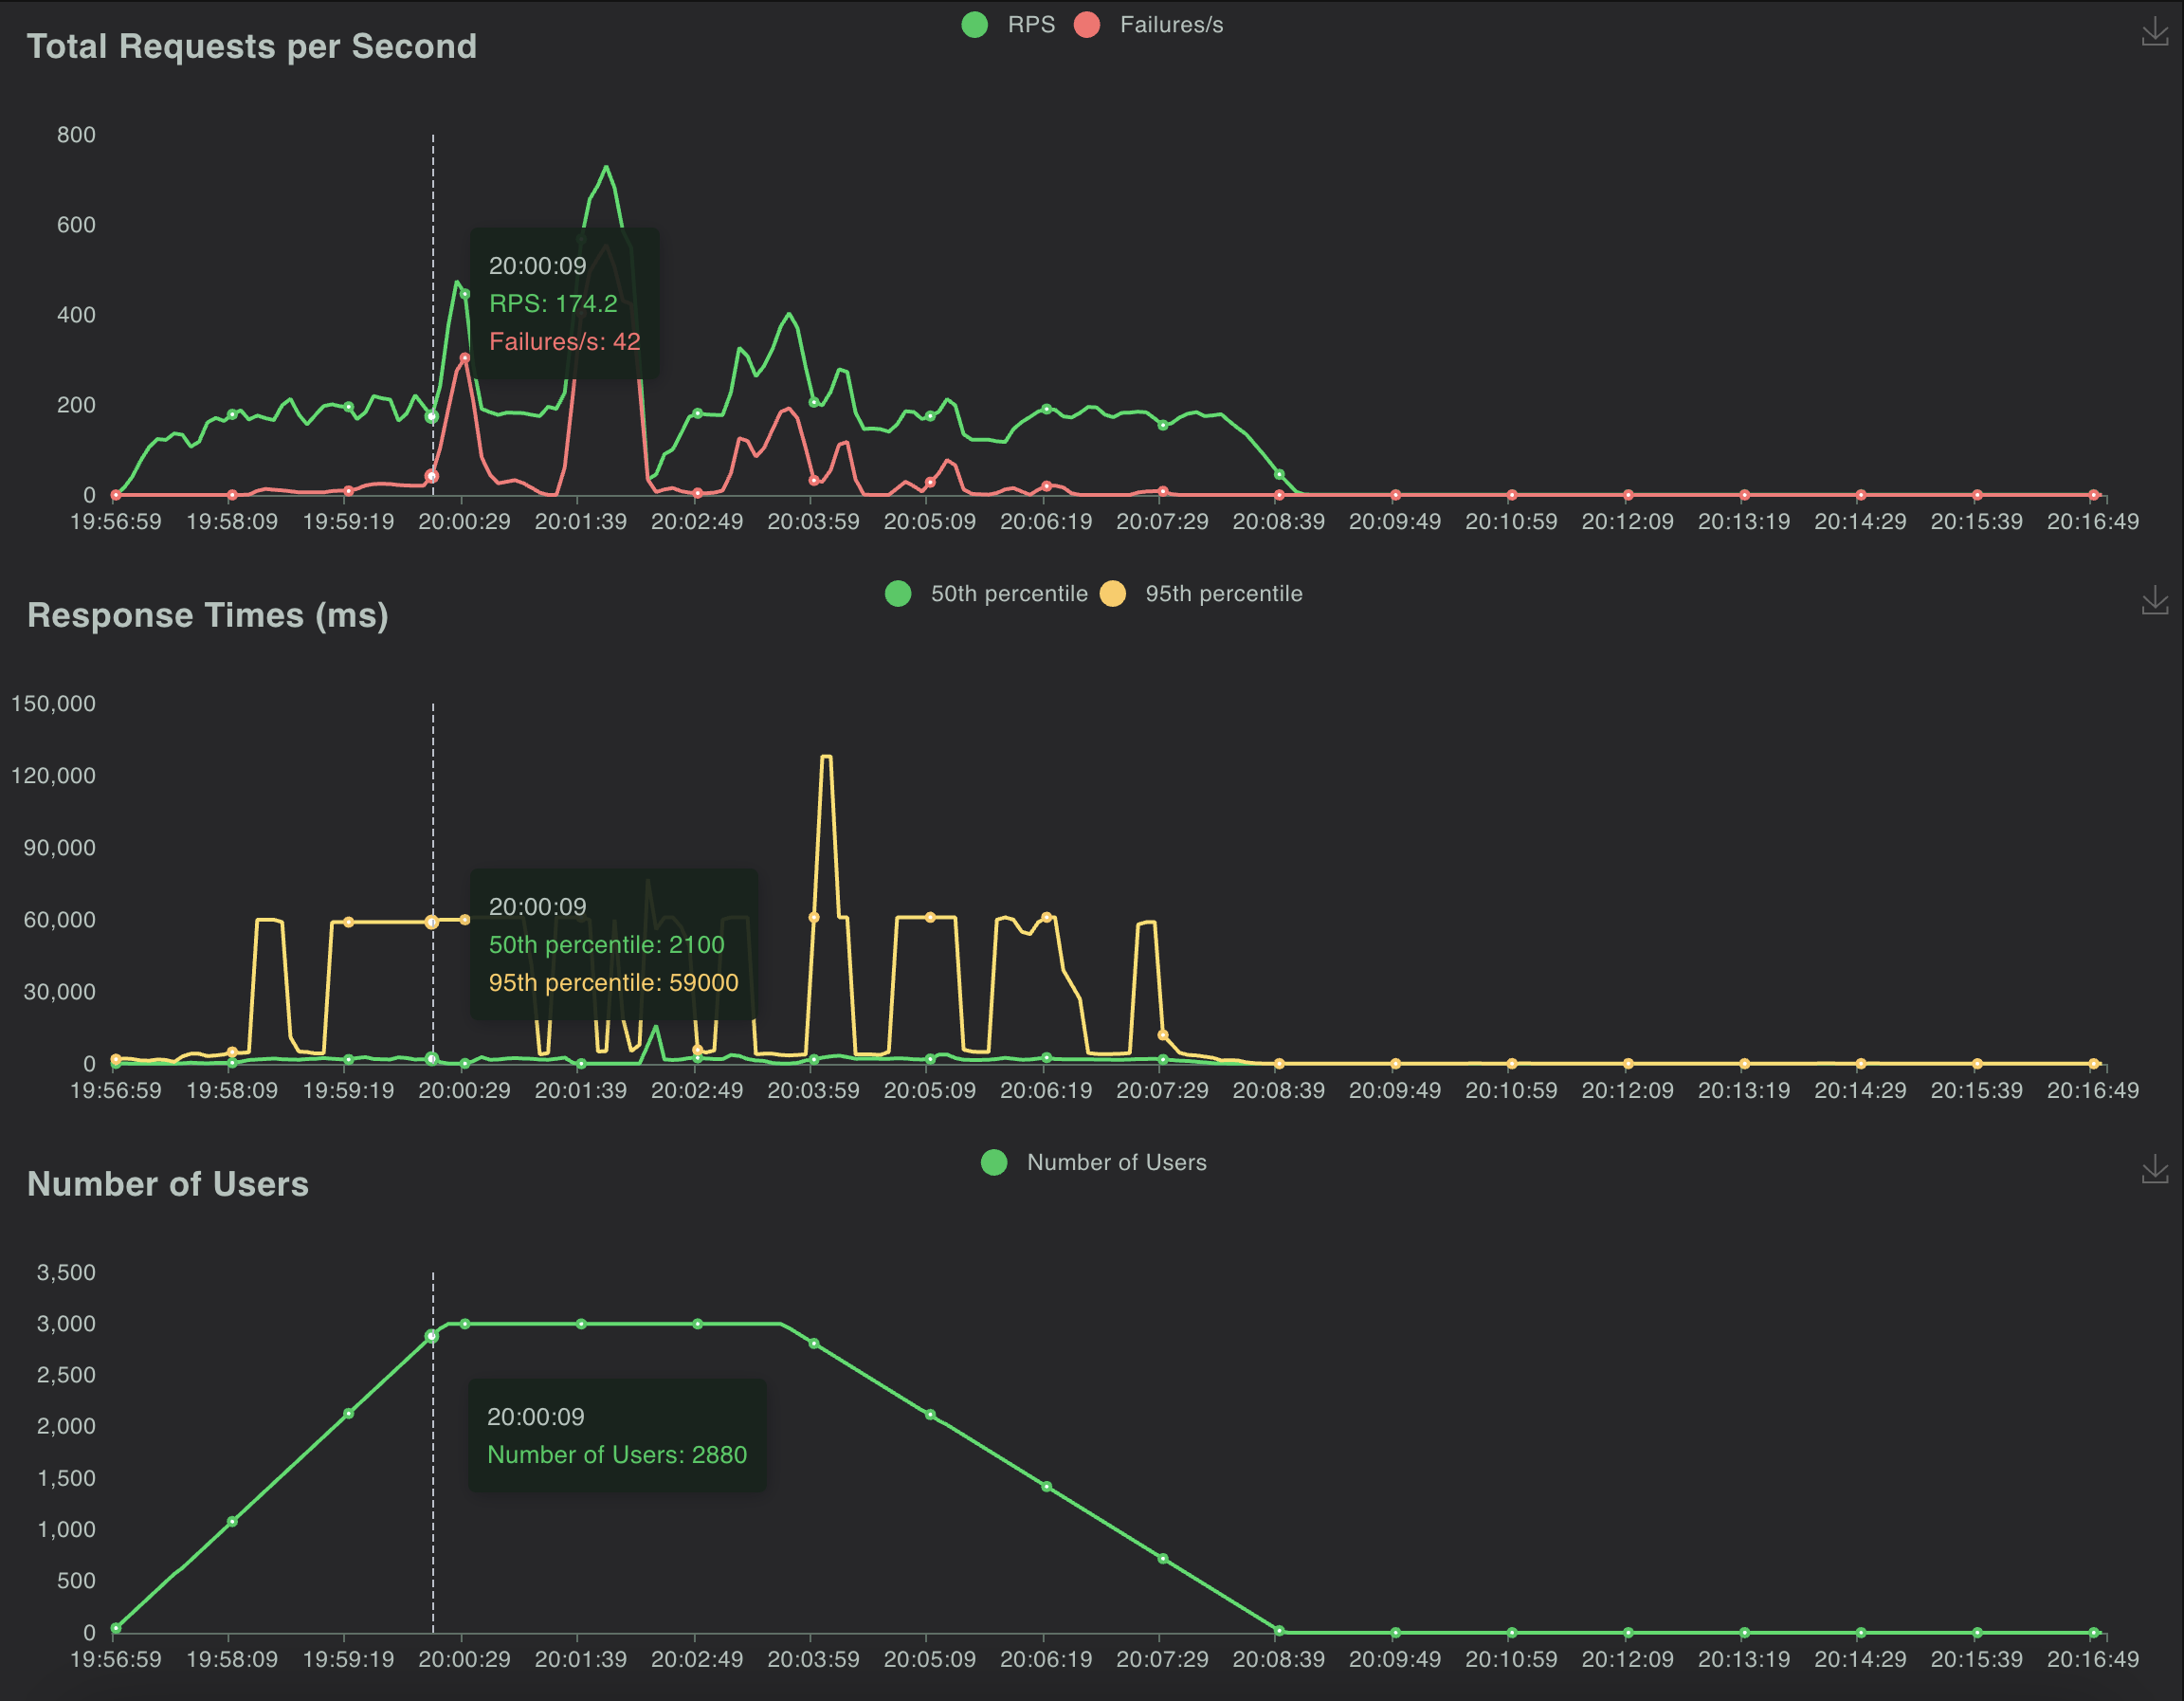
\includegraphics[width=0.9\linewidth]{images/exp2_results.png}
\end{figure}
We can see some initial failures that happen while auto scaling is happening. It takes a few moments to spawn up new pods / containers. The auto scaling still triggers failures as we approach the peak (after 2880 concurrent users). But as we keep decreasing the load, it manages to scale down and satisfy a lot of requests. Overall the failure \% is less compared to the case without any auto scaling. We can see that this satisfies the TR2. 


\subsubsection{Experiment 3: With Auto-Scaling (Exponential Load)}
In this case, we experiment by manually increasing the load exponentially. Because the load is exponentially increasing, we choose to user $t3.medium$ instances as opposed to $t3.micro$ instance in the previous experiment. We can then compare the results of this one with experiment 1 conducted with similar instances but without auto scaling. We can see that with auto scaling enabled on $t3.medium$ instances, we can handle almost 10000 concurrent users with very minimal failures. (As opposed to about 3000 users without autoscaling). We can also see the autoscaler in action and events, quickly adjusting to load in the figures below. 
\\\\
Hence, we observed the best performance with autoscaler enabled running on Autoscaling Node Group with $t3.medium$ instances that could handle exponentially increasing load really well.  We can see that this satisfies the TR2. We have enabled auto scaling using HPA and seen that even with exponential increase in load, $t3.medium$ instances are able to handle load really well.  
\\\\
Below are some screenshots of the results. 
\begin{figure}[H]
    \centering
    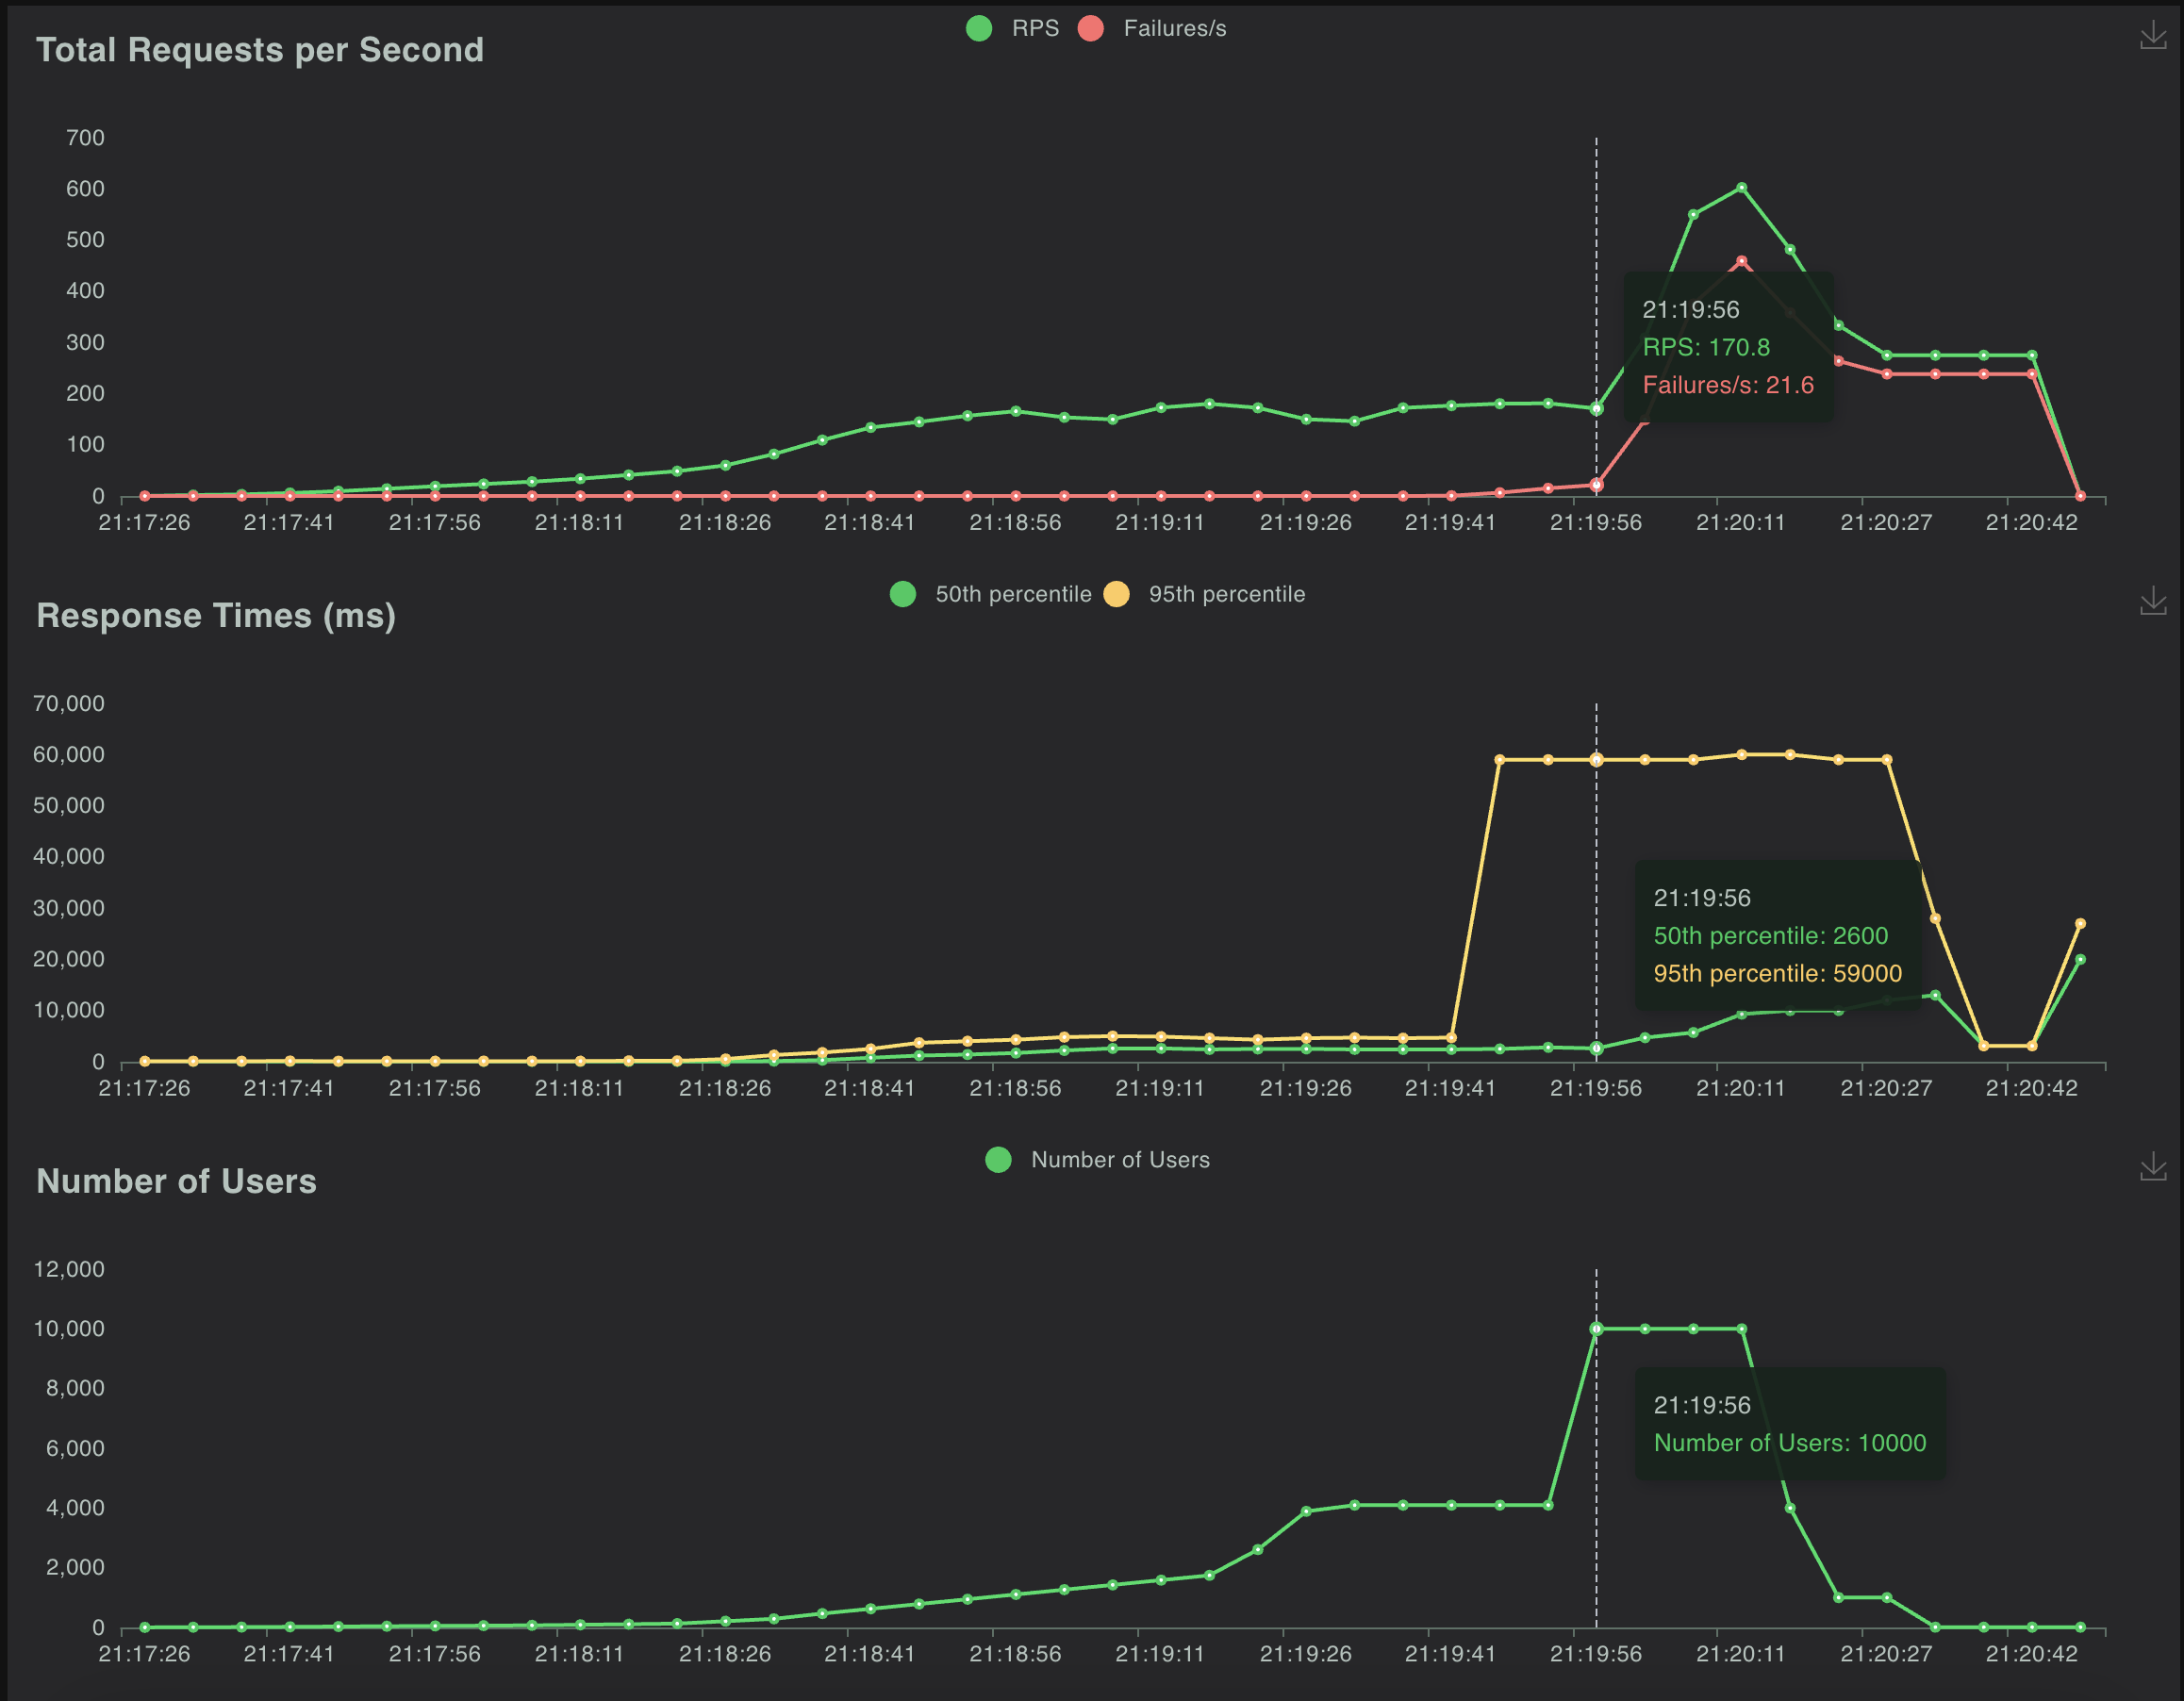
\includegraphics[width=\linewidth]{images/exp3_results.png}
    \label{exp3}
\end{figure}

\begin{figure}[H]
    \centering
    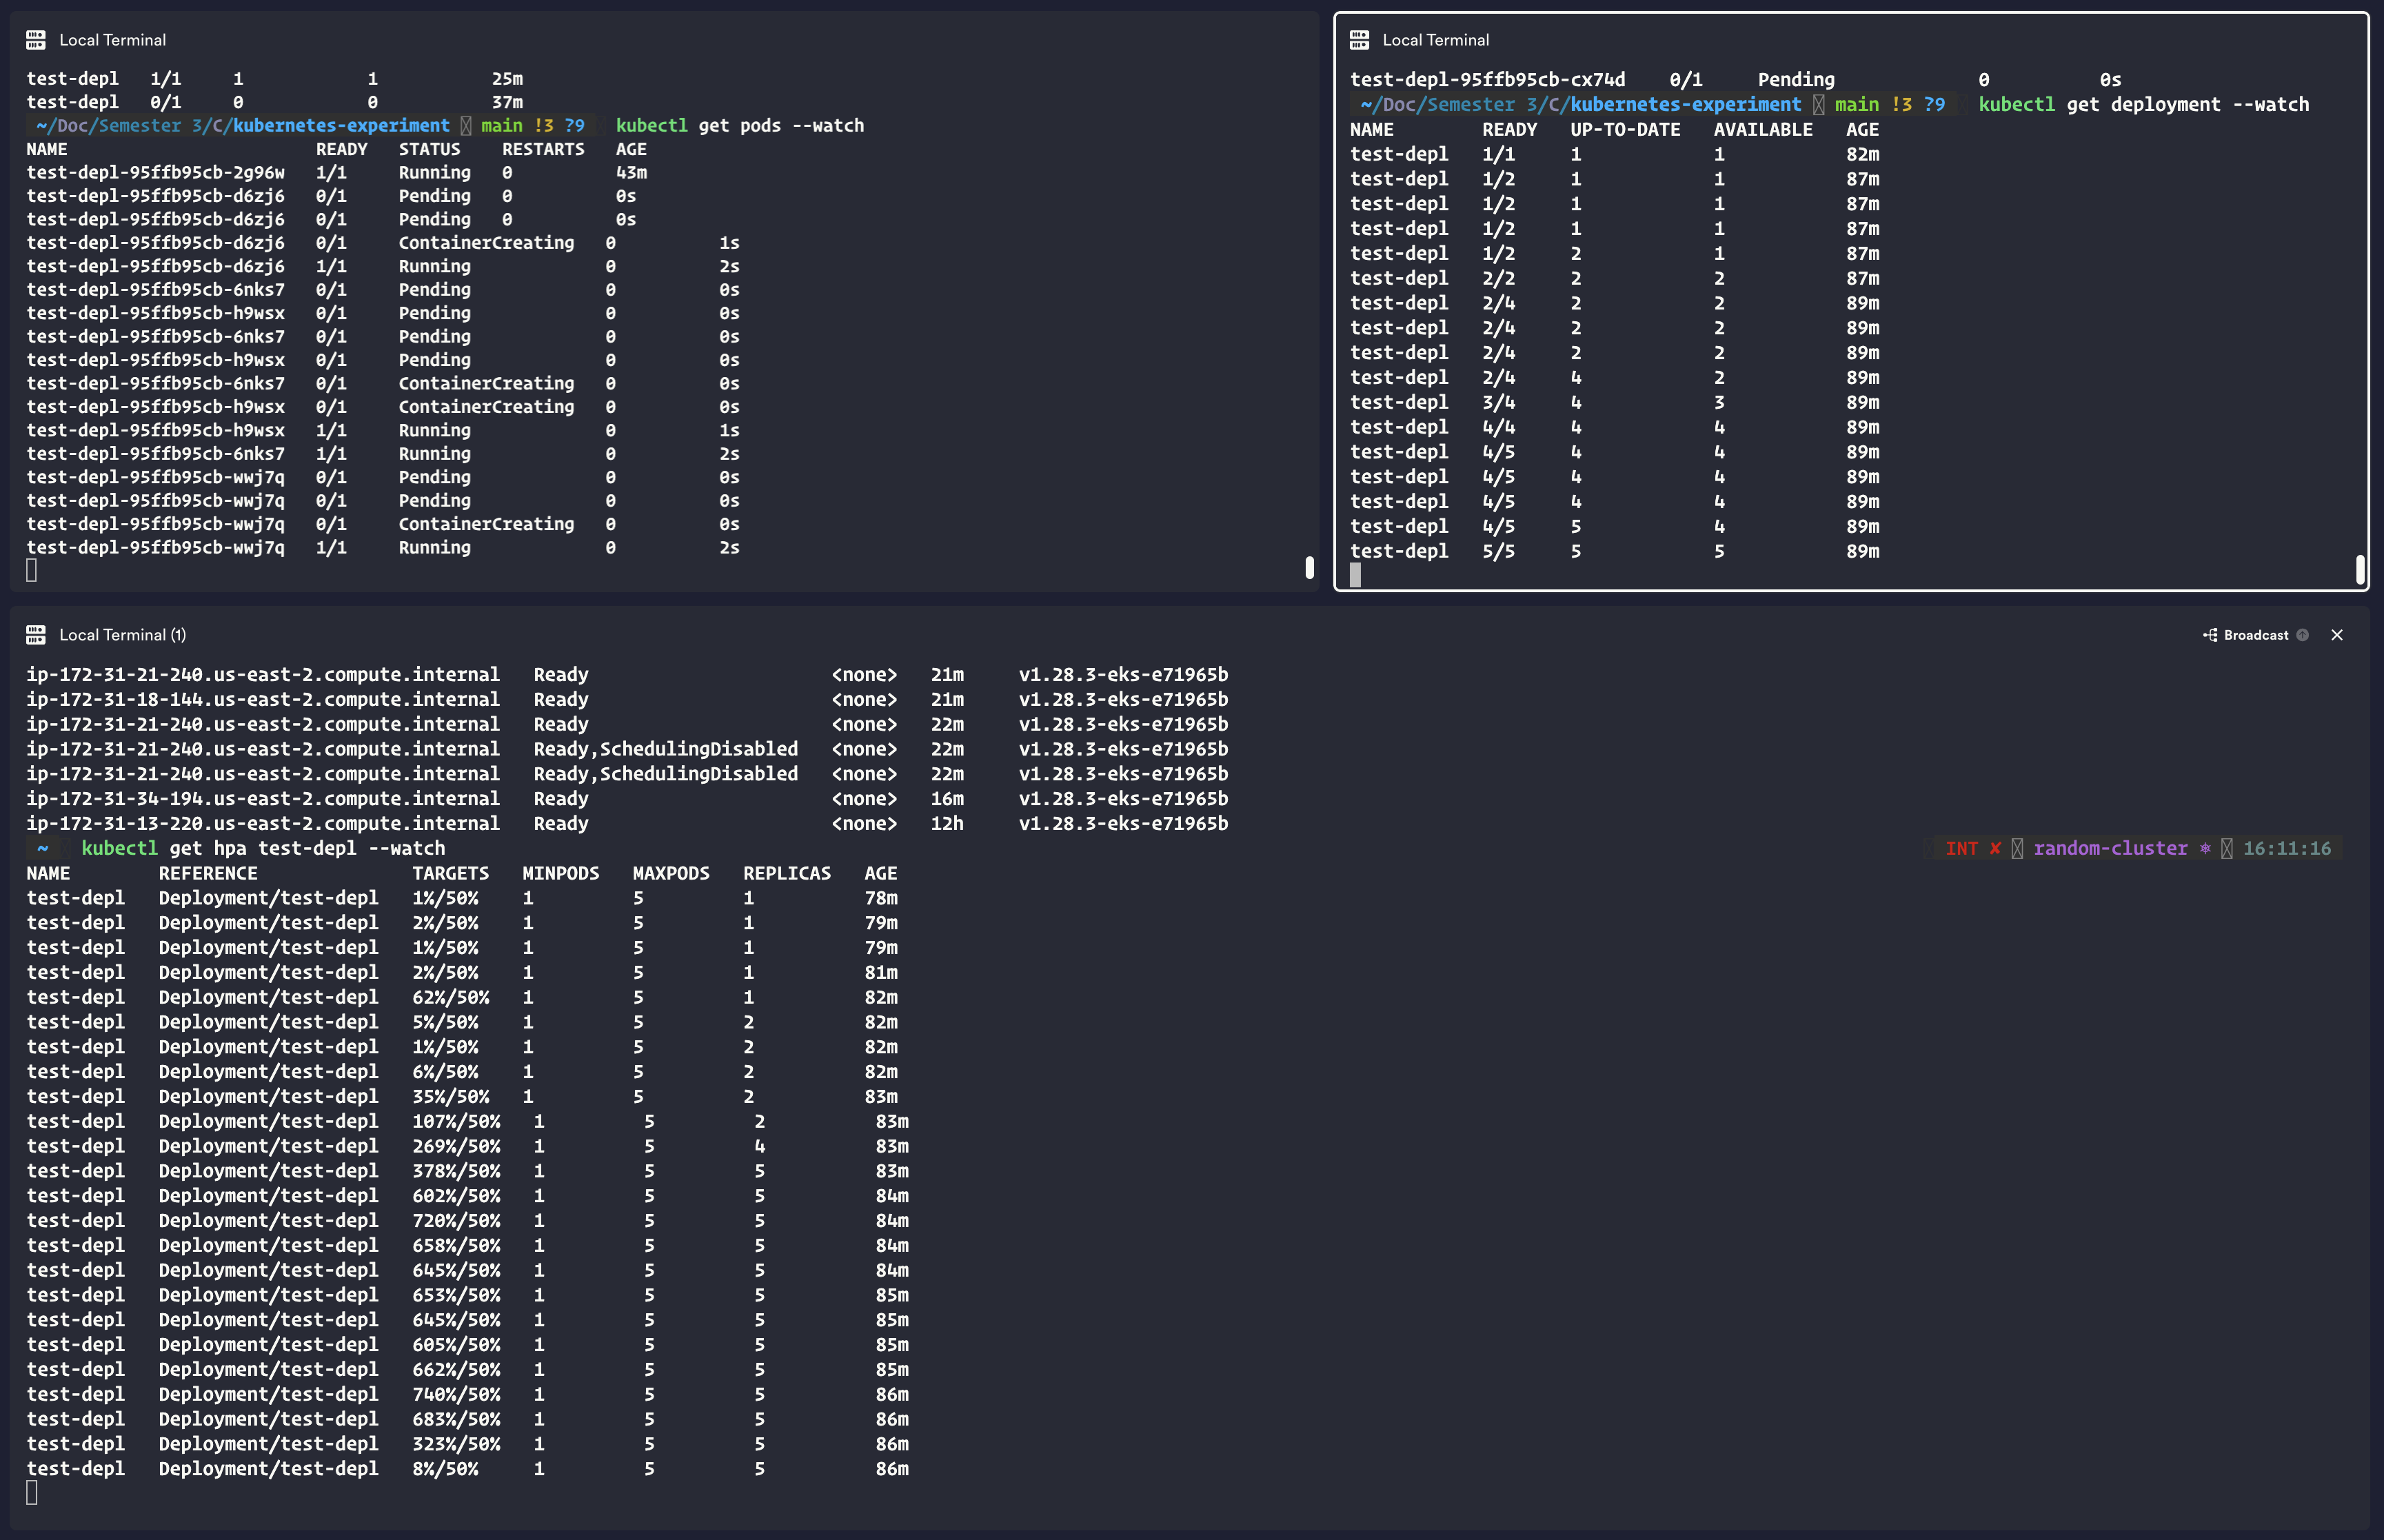
\includegraphics[width=0.9\linewidth]{images/exp3_watch.png}
\end{figure}
\begin{figure}[H]
    \centering
    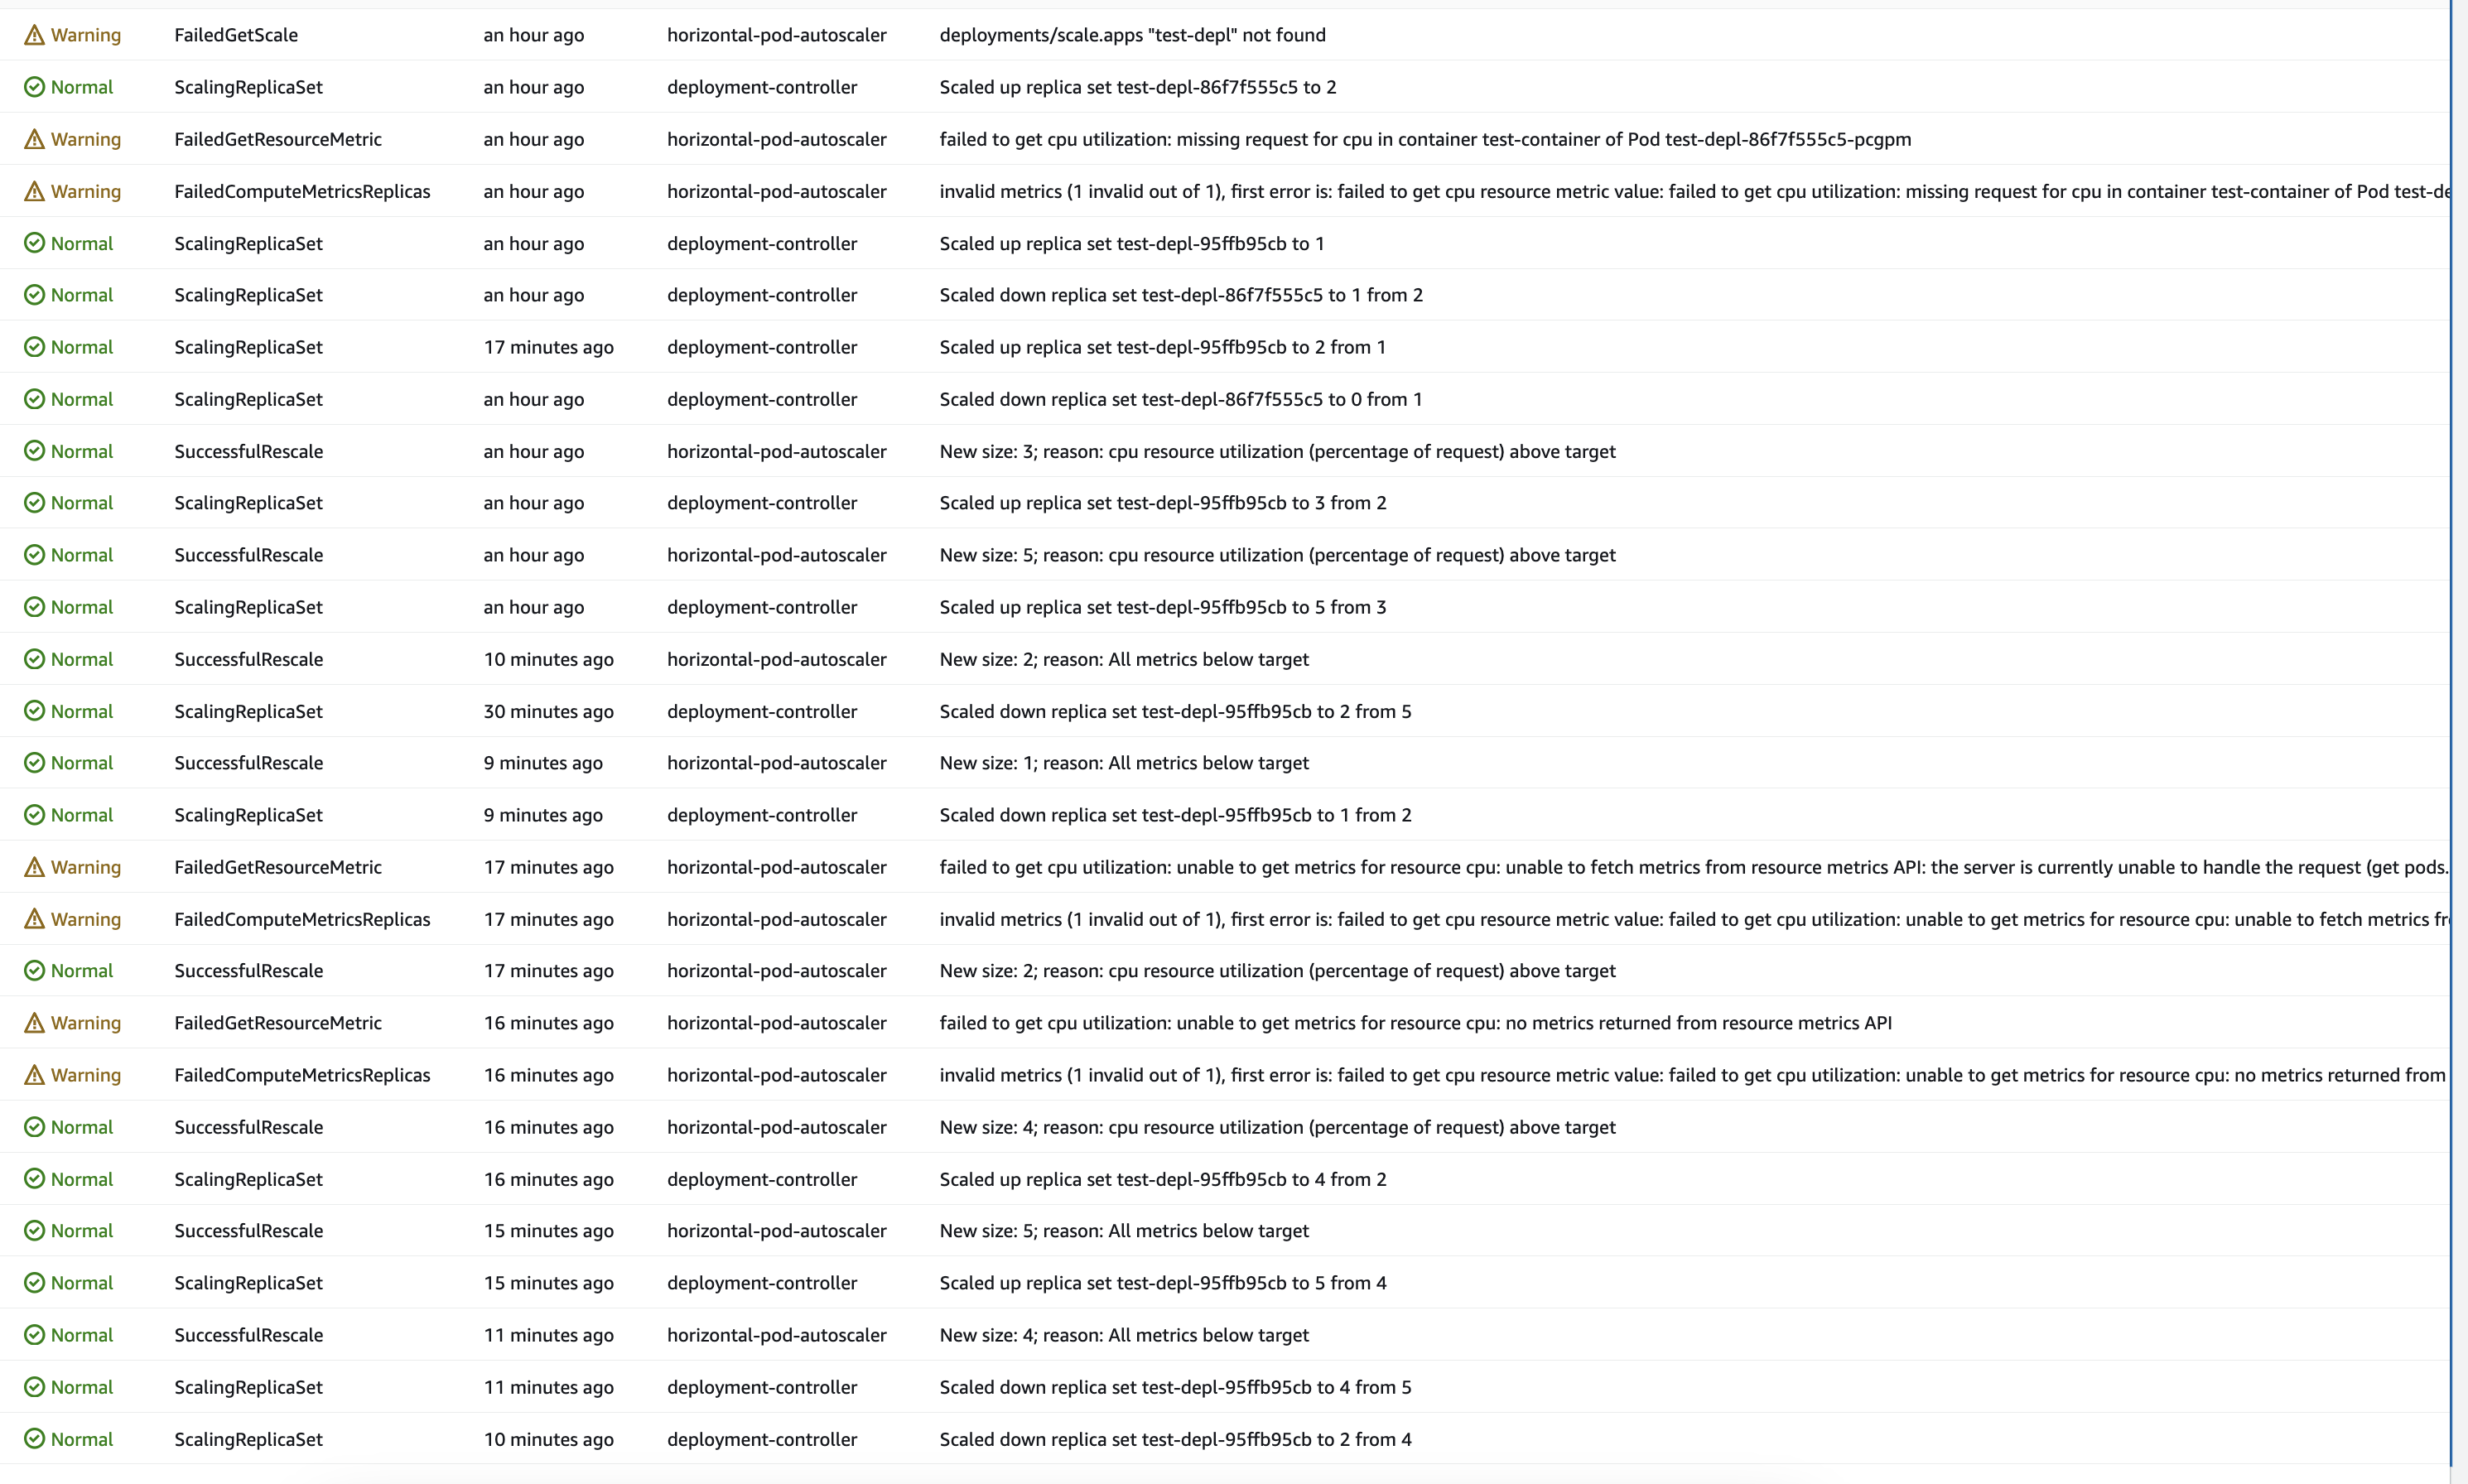
\includegraphics[width=0.9\linewidth]{images/autoscaler_events.png}
\end{figure}
\newpage
\section{Ansible playbooks \color{red}[Skipped]}
\section{Demonstration \color{red}[Skipped]}
\section{Comparisons \color{red}[Skipped]}
\newpage
\section{Conclusion}
This cloud architecture project was a complex and challenging endeavor that required careful planning, critical decision-making, and continuous iteration. The project began by clearly defining the problem that needed to be solved, taking into account both business and technical requirements. Choosing a cloud provider was a critical decision that had a significant impact on the project's success. The provider was selected based on a set of predefined criteria and a detailed comparison of different options. The chosen provider not only met the project's requirements but also offered a suite of services that were essential for the project's success. \\\\ 
The project's design evolved over time, from a simple initial design to a complex and detailed blueprint. The design was based on the AWS Well-Architected Framework and incorporated best practices for scalability, security, and reliability. We also experimented with Kubernetes to validate the scalability an application. These experiments proved how autoscaling (pod and node combined) could handle varying loads effectively, which is important for real-world implementation.\\\\
In conclusion, this project was a valuable learning experience that taught us a lot about designing cloud architectures. We understood the importance of using structured methodologies, validating designs thoroughly, and considering trade-offs carefully. The lessons learned from this project will be valuable for future projects. Some of them are listed below:
\subsection{The lessons learned}
\begin{enumerate}
    \item \textbf{Define the problem clearly:} Before starting any cloud architecture project, it is important to clearly define the problem that needs to be solved. This will help to ensure that the project is focused on the right requirements and that the chosen solution is the best fit for the problem.
    \item \textbf{Choose a cloud provider carefully:} The selection of a cloud provider is a critical decision that can have a significant impact on the project's success. It is important to carefully evaluate different providers and select one that meets the project's requirements and offers the services that are needed.

    \item \textbf{Use a structured methodology:} There are a number of different structured methodologies that can be used to design cloud architectures. Using a structured methodology will help to ensure that the design is well-thought-out and that all requirements are met.

    \item \textbf{Validate designs thoroughly:} It is important to validate cloud architecture designs thoroughly to ensure that they are scalable, secure, and reliable. This can be done through a variety of methods, such as testing, modeling, and simulation.

    \item \textbf{Consider trade-offs carefully:} There are often tradeoffs that need to be considered when designing cloud architectures. For example, there is often a trade-off between scalability and cost. It is important to carefully consider these tradeoffs and make decisions that are in the best interests of the organization.

    \item \textbf{Use the AWS Well-Architected Framework:} The AWS Well-Architected Framework is a valuable resource for designing cloud architectures. The framework provides a set of best practices that can help to ensure that architectures are scalable, secure, efficient, cost-effective, and reliable.

    \item \textbf{Experiment with Kubernetes:} Kubernetes is a container orchestration platform that can be used to manage containerized applications in the cloud. Experimenting with Kubernetes can help to validate the scalability of a cloud architecture.

    \item \textbf{Continuously assess and improve:} Cloud architectures are not static. They need to be continuously assessed and improved to meet the changing needs of the organization.

    \item \textbf{Document the architecture:} It is important to document the cloud architecture so that it can be easily understood and maintained.

    \item \textbf{Learn from mistakes:} Everyone makes mistakes, and this is especially true when designing cloud architectures. It is important to learn from mistakes and make sure that they are not repeated in future projects.
\end{enumerate}
\subsection{Possible continuation of the project \color{red}[Skipped]}
\newpage
\begin{thebibliography}{9}

\bibitem{Auto-Scaling} \href{https://www.cloudkeeper.com/insights/blogs/aws-auto-scaling-cost-optimization-practices-strategies#:~:text=Here%20are%20some%20best%20practices,sure%20you%20have%20the}{Cost Optimization with AWS Auto Scaling}

\bibitem{Health check} \href{https://www.cloudfoundry.org/blog/health-check-apps-cloud-part-1/#:~:text=,some%20sort%20of%20health%20checking}{Health Checks}
\bibitem{Budget} \href{https://www.xenonstack.com/insights/budget-alarms-in-aws#:~:text=,com%E3%80%91}{Budgeting Alerts}
\bibitem{multi-tenancy} \href{https://aws.amazon.com/blogs/architecture/lets-architect-multi-tenant-saas-architectures/}{Designing architectures for multi-tenancy}
\bibitem{IAM} \href{https://www.matillion.com/blog/role-based-access-control-rbac-in-the-cloud-iam-roles-matillion}{RBAC in Cloud}
\bibitem{MQTT} \href{https://event.moxa.com/newsletter/connection/2019/10/feat_02.html#:~:text=Message%20Queuing%20Telemetry%20Transport%20,cloud%20and%20cloud%20to%20device}{MQTT Is Important for Edge-to-cloud Connectivity}
\bibitem{Logging} \href{https://bluexp.netapp.com/blog/cis-blg-cloud-logging-strategies-for-multi-cloud-environments#:~:text=,events%20occurring%20in%20your%20systems}{Cloud Logging}
\bibitem{Encryption} \href{https://link.springer.com/chapter/10.1007/978-3-030-52243-8_17#:~:text=Specifically%2C%20we%20design%20and%20demonstrate,encryption%2C%20in%20order%20to}{Secure Aerial Data Delivery with Lightweight Encryption}

\bibitem {Auto-Scaling for High Availability} \href{https://www.cloudlaya.com/blog/using-auto-scaling-and-load-balancing-for-high-availability/}{Auto-Scaling for High Availability}

\bibitem {rate} \href{https://www.solo.io/topics/rate-limiting/}{Rate Limiting and DOS Atttack}

\bibitem {version control} \href{https://www.linkedin.com/pulse/high-availability-disaster-recovery-plan-version-control-kosiec/}{High Availability and Disaster Recovery Plan for Version Control System}

\bibitem {HA} \href{https://youtu.be/opxEYVcsubk?si=QCq5AcQ3x9gB4NVe}{Video on Regular Health Checks To Ensure High Availability}

\bibitem {multi-region architecture} \href{https://www.cockroachlabs.com/blog/multi-region-architecture-ha/}{multi-region architecture: The key to high availability & risk mitigation}

% \bibitem {cloudfront} \href{https://docs.aws.amazon.com/cloudfront/}{Amazon CloudFront Documentation}

\bibitem {Delayed data} \href{https://journals.sagepub.com/doi/10.1177/15501329221097815#}{Delay-reliability-aware protocol adaption}

\bibitem {quicksight} \href{https://docs.aws.amazon.com/quicksight//}{Amazon Quicksight Documentation}

\bibitem{grafana}
\href{https://docs.aws.amazon.com/grafana/}{Amazon Managed Grafana Documentation}

\bibitem{s3}
\href{https://docs.aws.amazon.com/s3/}{Amazon S3 Documentation}

\bibitem {cloudfront} \href{https://docs.aws.amazon.com/cloudfront/}{Amazon CloudFront Documentation}

\bibitem {apigateway} \href{https://docs.aws.amazon.com/apigateway/}{Amazon API Gateway Documentation}

\bibitem{wafirewall} 
\href{https://docs.aws.amazon.com/waf/}{AWS WAF Documentation}

\bibitem{ecs}
\href{https://docs.aws.amazon.com/ecs/}{Amazon ECS Documentation}
\bibitem{lambda} \href{https://docs.aws.amazon.com/lambda/}{AWS Lambda Documentation}

\bibitem{alb} \href{https://docs.aws.amazon.com/elasticloadbalancing/latest/application/introduction.html}{AWS Application Load Balancer Documentation}

\bibitem{kms}
\href{https://docs.aws.amazon.com/kms/}{AWS KMS Documentation}

\bibitem{dynamo}
\href{https://docs.aws.amazon.com/dynamodb/}{Amazon DynamoDB Documentation}


\bibitem{cloudwatch}
\href{https://docs.aws.amazon.com/cloudwatch/}{Amazon Cloudwatch Documentation}

\bibitem{elcache} \href{https://docs.aws.amazon.com/elasticache/}{Amazon ElastiCache Documentation}

\bibitem{iot}
\href{https://docs.aws.amazon.com/iot-core/}{AWS IoT Core Documentation}

\bibitem{route53} \href{https://docs.aws.amazon.com/route53/}{AWS Route 53 Documentation}

\bibitem{costexplore}
\href{https://docs.aws.amazon.com/cost-explorer/}{AWS Cost Explorer Documentation}

\bibitem{budgets} \href{https://docs.aws.amazon.com/awsaccountbilling/}{AWS Budgets Documentation}

\bibitem{kinesis}
\href{https://docs.aws.amazon.com/kinesis/}{Amazon Kinesis Documentation}

\bibitem{ec2}
\href{https://docs.aws.amazon.com/ec2/}{Amazon EC2 Documentation}

\bibitem{autoscale} \href{https://docs.aws.amazon.com/autoscaling/}{AWS Auto Scaling Documentation}

\bibitem{IAM} \href{https://docs.aws.amazon.com/iam/}{AWS  Identity and Access Managemen Documentation}

\bibitem{microservices}\href{https://aws.amazon.com/microservices/}{What are Microservices?}


\bibitem{nextcloud}
\href{https://nextcloud.com/}{NextCloud Home Page}

\bibitem{locust}
\href{https://locust.io/}{Locust Official Website}

\bibitem{locust_docs} \href{https://docs.locust.io/en/stable/}{Locust Documentation}

\bibitem{lambda_events} 
\href{https://docs.aws.amazon.com/lambda/latest/dg/lambda-services.html#event-driven-invocation}{AWS Lambda - Event-driven invocation}

\bibitem{iam}
\href{https://aws.amazon.com/iam/}{AWS IAM Documentation}

\bibitem{ses}
\href{https://aws.amazon.com/ses/}{AWS Simple Email Service (SES) Documentation}

\bibitem{Operational Excellence}
\href{https://docs.aws.amazon.com/wellarchitected/latest/operational-excellence-pillar/welcome.html}{AWS Operational Excellence Pillar whitepaper}

\bibitem{Security}
\href{https://docs.aws.amazon.com/wellarchitected/latest/security-pillar/welcome.html}{AWS Security Pillar whitepaper}

\bibitem{Reliability}
\href{https://docs.aws.amazon.com/wellarchitected/latest/reliability-pillar/welcome.html}{AWS Reliability Pillar whitepaper}

\bibitem{Performance}
\href{https://docs.aws.amazon.com/wellarchitected/latest/performance-efficiency-pillar/welcome.html}{AWS Performance Efficiency Pillar whitepaper}

\bibitem{Cost Optimization}
\href{https://docs.aws.amazon.com/wellarchitected/latest/cost-optimization-pillar/welcome.html}{AWS Cost Optimization Pillar whitepaper}

\bibitem{Sustainability}
\href{https://docs.aws.amazon.com/wellarchitected/latest/sustainability-pillar/welcome.html}{AWS Sustainability Pillar whitepaper}

\bibitem{Opex}
\href{https://docs.aws.amazon.com/wellarchitected/latest/framework/oe-design-principles.html}{Design Principle Operational excellence}

\bibitem{rel}
\href{https://docs.aws.amazon.com/wellarchitected/latest/framework/rel-dp.html}{Design Principle Reliability}

\bibitem{Cost dp}
\href{https://docs.aws.amazon.com/wellarchitected/latest/framework/cost-dp.html}{Design Principle Cost}


\bibitem{prepare}
\href{https://docs.aws.amazon.com/wellarchitected/latest/framework/oe-prepare.html}{Best Practices Prepare}

\bibitem{operate}
\href{https://docs.aws.amazon.com/wellarchitected/latest/framework/oe-operate.html}{Best Practices Operate}

\bibitem{evolve}
\href{https://docs.aws.amazon.com/wellarchitected/latest/framework/oe-evolve.html}{Best Practices Evolve}

\bibitem{identity}
\href{https://docs.aws.amazon.com/wellarchitected/latest/framework/sec-iam.html}{Best Practices Iam}

\bibitem{Infrastructure protection}
\href{https://docs.aws.amazon.com/wellarchitected/latest/framework/sec-infrastructure.html}{Best Practices Infrastructure protection}

\bibitem{Data protection}
\href{https://docs.aws.amazon.com/wellarchitected/latest/framework/sec-dataprot.html}{Best Practices Data protection}

\bibitem{Incident response}
\href{https://docs.aws.amazon.com/wellarchitected/latest/framework/sec-incresp.html}{Best Practices Incident response}

\bibitem{Failure management}
\href{https://docs.aws.amazon.com/wellarchitected/latest/framework/rel-failmgmt.html}{Best Practices Failure management}

\bibitem{Foundations}
\href{https://docs.aws.amazon.com/wellarchitected/latest/framework/rel-found.html}{Best Practices Foundations}

\bibitem{monitoring}
\href{https://docs.aws.amazon.com/wellarchitected/2022-03-31/framework/perf-monitoring.html}{Best Practices monitoring}

\bibitem{Expenditure and usage awareness}
\href{https://docs.aws.amazon.com/wellarchitected/latest/framework/cost-aware.html}{Best Practices Expenditure and usage awareness}

\bibitem{Manage demand and supply resources}
\href{https://docs.aws.amazon.com/wellarchitected/latest/framework/cost-mandem.html}{Best Practices Manage demand and supply resources}



\end{thebibliography}
\end{document}
